

\documentclass{Configuration_Files/PoliMi3i_thesis}

% CONFIGURATIONS
\usepackage{parskip} % For paragraph layout
\usepackage{setspace} % For using single or double spacing
\usepackage{emptypage} % To insert empty pages
\usepackage{multicol} % To write in multiple columns 
\setlength\columnsep{15pt} % Column separation in executive summary
\setlength\parindent{0pt} % Indentation

\raggedbottom  

% PACKAGES FOR TITLES
\usepackage{titlesec}
\titlespacing{\section}{0pt}{3.3ex}{2ex}
\titlespacing{\subsection}{0pt}{3.3ex}{1.65ex}
\titlespacing{\subsubsection}{0pt}{3.3ex}{1ex}
\usepackage{color}

% PACKAGES FOR LANGUAGE AND FONT
\usepackage[english]{babel} % The document is in English  
\usepackage[utf8]{inputenc} % UTF8 encoding
\usepackage[T1]{fontenc} % Font encoding
\usepackage[11pt]{moresize} % Big fonts

% PACKAGES FOR IMAGES
\usepackage{graphicx}
\usepackage{transparent} % Enables transparent images
\usepackage{eso-pic} % For the background picture on the title page
\usepackage{subfig} % Numbered and caption subfigures using 
\usepackage{tikz} % A package for high-quality hand-made figures.
\usetikzlibrary{}
\graphicspath{{./Images/}} % Directory of the images
\usepackage{caption} % Coloured captions
\usepackage{xcolor} % Coloured captions
\usepackage{amsthm,thmtools,xcolor} % Coloured "Theorem"
\usepackage{float}

% STANDARD MATH PACKAGES
\usepackage{amsmath}
\usepackage{amsthm}
\usepackage{amssymb}
\usepackage{amsfonts}
\usepackage{bm}
\usepackage[overload]{empheq} % For braced-style 
\usepackage{fix-cm} % To override original LaTeX restrictions 

% PACKAGES FOR TABLES
\usepackage{longtable} % Pacchetto per tabelle multi-pagina
\usepackage{tabularx} % Pacchetto per tabelle adattabili
\usepackage{array} % Pacchetto per definire nuovi tipi di colonna
\usepackage{caption} % Pacchetto per gestire la didascalia
\usepackage{geometry}
\usepackage{colortbl}

% PACKAGES FOR ALGORITHMS (PSEUDO-CODE)
\usepackage{algorithm}
\usepackage{algorithmic}

% for sequence diagram
\usepackage{pgf-umlcd}
\usepackage{tikz}
\usetikzlibrary{arrows.meta, positioning}

% PACKAGES FOR REFERENCES & BIBLIOGRAPHY
\usepackage[colorlinks=true,linkcolor=black,anchorcolor=black,citecolor=black,filecolor=black,menucolor=black,runcolor=black,urlcolor=black]{hyperref} % Adds clickable links at references
\usepackage{cleveref}
\usepackage[square, numbers, sort&compress]{natbib} % Square brackets, citing references with numbers, citations sorted by appearance in the text and compressed
\bibliographystyle{abbrvnat} % You may use a different style adapted to your field

% OTHER PACKAGES
\usepackage{pdfpages} % To include a pdf file
\usepackage{afterpage}
\usepackage{lipsum} % DUMMY PACKAGE
\usepackage{fancyhdr} % For the headers
\fancyhf{}

\usepackage{listings}
\usepackage{xcolor}

% Define blue color typical of polimi
\definecolor{bluepoli}{cmyk}{0.4,0.1,0,0.4}

% Custom theorem environments
\declaretheoremstyle[
  headfont=\color{bluepoli}\normalfont\bfseries,
  bodyfont=\color{black}\normalfont\itshape,
]{colored}

% Set-up caption colors
\captionsetup[figure]{labelfont={color=bluepoli}} % Set colour of the captions
\captionsetup[table]{labelfont={color=bluepoli}} % Set colour of the captions
\captionsetup[algorithm]{labelfont={color=bluepoli}} % Set colour of the captions

\theoremstyle{colored}
\newtheorem{theorem}{Theorem}[chapter]
\newtheorem{proposition}{Proposition}[chapter]

% Enhances the features of the standard "table" and "tabular" environments.
\newcommand\T{\rule{0pt}{2.6ex}}
\newcommand\B{\rule[-1.2ex]{0pt}{0pt}}

% Pseudo-code algorithm descriptions.
\newcounter{algsubstate}
\renewcommand{\thealgsubstate}{\alph{algsubstate}}
\newenvironment{algsubstates}
  {\setcounter{algsubstate}{0}%
   \renewcommand{\STATE}{%
     \stepcounter{algsubstate}%
     \Statex {\small\thealgsubstate:}\space}}
  {}

% New font size
\newcommand\numfontsize{\@setfontsize\Huge{200}{60}}

% Title format: chapter
\titleformat{\chapter}[hang]{
\fontsize{50}{20}\selectfont\bfseries\filright}{\textcolor{bluepoli} \thechapter\hsp\hspace{2mm}\textcolor{bluepoli}{|   }\hsp}{0pt}{\huge\bfseries \textcolor{bluepoli}
}

% Title format: section
\titleformat{\section}
{\color{bluepoli}\normalfont\Large\bfseries}
{\color{bluepoli}\thesection.}{1em}{}

% Title format: subsection
\titleformat{\subsection}
{\color{bluepoli}\normalfont\large\bfseries}
{\color{bluepoli}\thesubsection.}{1em}{}

% Title format: subsubsection
\titleformat{\subsubsection}
{\color{bluepoli}\normalfont\large\bfseries}
{\color{bluepoli}\thesubsubsection.}{1em}{}

% Shortening for setting no horizontal-spacing
\newcommand{\hsp}{\hspace{0pt}}

\makeatletter
% Renewcommand: cleardoublepage including the background pic
\renewcommand*\cleardoublepage{%
  \clearpage\if@twoside\ifodd\c@page\else
  \null
  \AddToShipoutPicture*{\BackgroundPic}
  \thispagestyle{empty}%
  \newpage
  \if@twocolumn\hbox{}\newpage\fi\fi\fi}
\makeatother

%For correctly numbering algorithms
\numberwithin{algorithm}{chapter}

%------------------------
%	BEGIN OF YOUR DOCUMENT
%-------------------------

\begin{document}

\fancypagestyle{plain}{%
\fancyhf{} % Clear all header and footer fields
\fancyhead[RO,RE]{\thepage} %RO=right odd, RE=right even
\renewcommand{\headrulewidth}{0pt}
\renewcommand{\footrulewidth}{0pt}}

%-------------------
%	TITLE PAGE
%-------------------
\pagestyle{empty} %
\frontmatter 
\puttitle{
	title=Students \& Companies, 
	name= Paone A. Pasqual M. Restelli M., 
	course=Software Engineering 2 Project,
	advisor= Prof. Camilli Matteo,
	academicyear={2024-25},  
} 
\startpreamble
\setcounter{page}{1} 

% TABLE OF CONTENTS
\thispagestyle{empty}
\tableofcontents % Table of contents 
\thispagestyle{empty}
\cleardoublepage

%--------------------
%	THESIS MAIN TEXT
%--------------------
\addtocontents{toc}{\vspace{2em}} 
\mainmatter 



% -----------------------
% INTRODUCTION SECTION
% -----------------------
\chapter{Introduction}

\section{Purpose}
This document represents the Design Document (DD). The purpose of the DD is to provide overall guidance to the architecture of the software product discussed in the RASD.

It contains the description of the architecture chosen to design the Students\&Companies web application. Furthermore, it describes how the UI will look like, and it maps the requirements defined in the RASD to the architectural components defined in this document.
It also includes a set of design characteristics required for the implementation by introducing constraints and quality attributes, and it gives a presentation of the implementation, integration, and testing plan.

The DD is addressed to the software development team who will have to implement the described system, and it has the purpose of guiding them through the development process.


\section{Scope}
Students \& Companies (S\&C) is a platform linking students with internship opportunities and corporations. Companies can advertise roles, get candidate recommendations, and send invitations. Students can search for roles actively or receive notifications for matches. Mutual interest brings to the selection process, composed of interviews, and possibly to an internship being carried out. During internships, S\&C gathers feedback, manages complaints, and involves universities when needed to resolve issues.

The platform is implemented using the 3-tier design pattern, a client-server software pattern that separates applications into three logical layers, each with distinct responsibilities.  
More implementation choices are covered in later sections of this document.


\pagebreak
\section{Definitions, Acronymous, Abbreviations}
\begin{table}[H]
\centering
\begin{tabular}{|l|l|}
\hline
\textbf{Abbreviation} & \textbf{Description} \\ \hline
RASD & Requirements Analysis \& Specification Document \\ \hline
DD & Design Document \\ \hline
G* & Goal \\ \hline
D* & Domain assumption \\ \hline
R* & Functional requirement \\ \hline
S\&C & Students \& Companies \\ \hline
STs & Students \\ \hline
COMs & Companies \\ \hline
UNs & Universities \\ \hline
UML & Unified Modelling Language \\ \hline
UI & User Interface \\ \hline
\end{tabular}
\caption{List of Definitions, Acronymous, and Abbreviations}
\label{table:abbreviations}
\end{table}

\section{Revision History}

\begin{itemize}
    \item Version 1.0 (07/01/2025)
\end{itemize}

\section{Reference Documents}

The document is based on the following materials:

\begin{itemize}
    \item IEEE Standard Documentation For DD
    \item The specification of the RASD and DD assignment of the Software Engineering II course a.a. 2024/25 
    \item Slides of the course on WeBeep
\end{itemize}

\pagebreak
\section{Document structure}
This document is composed of six chapters:
\begin{enumerate}
    \item \textbf{ Introduction:} This chapter describes the scope and purpose of this DD. It also includes the structure of the document and a set of definitions, acronyms, and abbreviations used.
    \item \textbf{ Architectural Design:} This chapter presents the architectural design choices. It includes an overview of the designed architecture, all the components, the interfaces, and the technologies used for designing the application. It also details the main functions of the interfaces and the processes in which they are utilized (Runtime view and component interfaces). Finally, it explains the design patterns chosen and recommended for system development.
    \item \textbf{User Interface Design:} This chapter illustrates how the UI should look. It complements and expands upon the User Interfaces subsection in the RASD.
    \item \textbf{Requirements Traceability.} This chapter explains how the requirements defined in the RASD are mapped to the design elements defined in this document.
    \item \textbf{Implementation, Integration, and Test Plan.} This chapter outlines the planned order for implementing the system's subcomponents, integrating them, and testing the integration.
    \item \textbf{Effort Spent.} This chapter provides information on the number of hours each group member has worked on this document.
\end{enumerate}


\chapter{Architectural Design}

\section{Overview}
We chose to design the Students\&Companies (S\&C) web application using a three-tier architecture with remote presentation. These three tiers correspond to a client tier, application tier, and data tier. The client (presentation) tier serves the needs of students, companies, and universities using the S\&C platform. The application layer is the one that processes user requests, performs statistical analysis, and interacts with the internal data tier. The data tier is responsible for data management and storage. It handles all database operations, including data retrieval, updates, and management. To better improve and ensure load distribution and scalability, it was chosen to implement a load balancer between the client and application layer, in particular inside the web server.

A 3-tier architecture is suitable for a career service application as it makes the system easier to manage and scale. It ensures reliability through load balancing, which helps handle high traffic during peak usage. This architecture supports advanced features like job matching and analytics, integrates well with cloud services, and provides flexibility for future updates, such as adding mobile apps or AI tools. Its structure also improves security by isolating sensitive data in the database layer. The S\&C architecture specializes in three different groups of components each with its own characteristics and responsibilities:
\begin{enumerate}
    \item \textbf{Presentation layer:} The Presentation (client) Tier is the application's front end, managing the user interface and interactions for data input and display. Its goal is to display data, collect inputs,and provide a seamless user experience. 
    \item \textbf{Application layer:} It handles tasks like user authentication, recommendation matching algorithms, managing user accounts, handling notifications, and communication between the user interface and the database.
    \item \textbf{Data layer}: Stores and manages critical data such as user profiles, student CVs, project descriptions, and application history. It ensures data security and efficient retrieval for real-time use in the application.
\end{enumerate}

\begin{figure}[H]
    \centering
    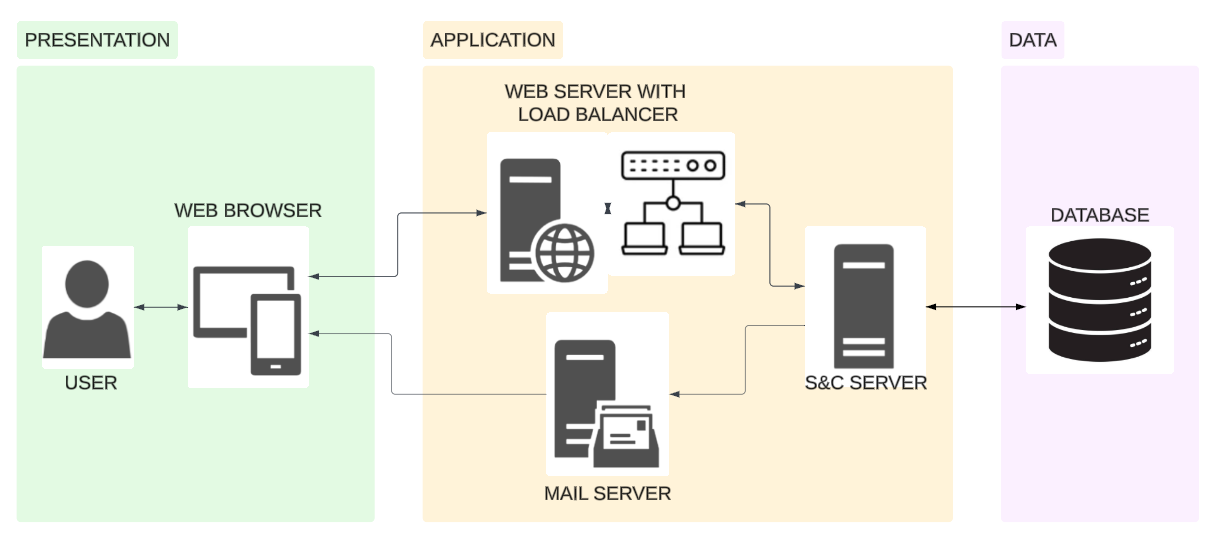
\includegraphics[width=0.9\linewidth]{DD//Images/3tier.png}
    \caption{High level architecture }
\end{figure}

\section{Component view: Component diagram}

Figure 2.2 presents a detailed diagram illustrating the components that constitute our application. Below is an explanation of each component and its purpose.

\begin{figure}[H]
    \centering
    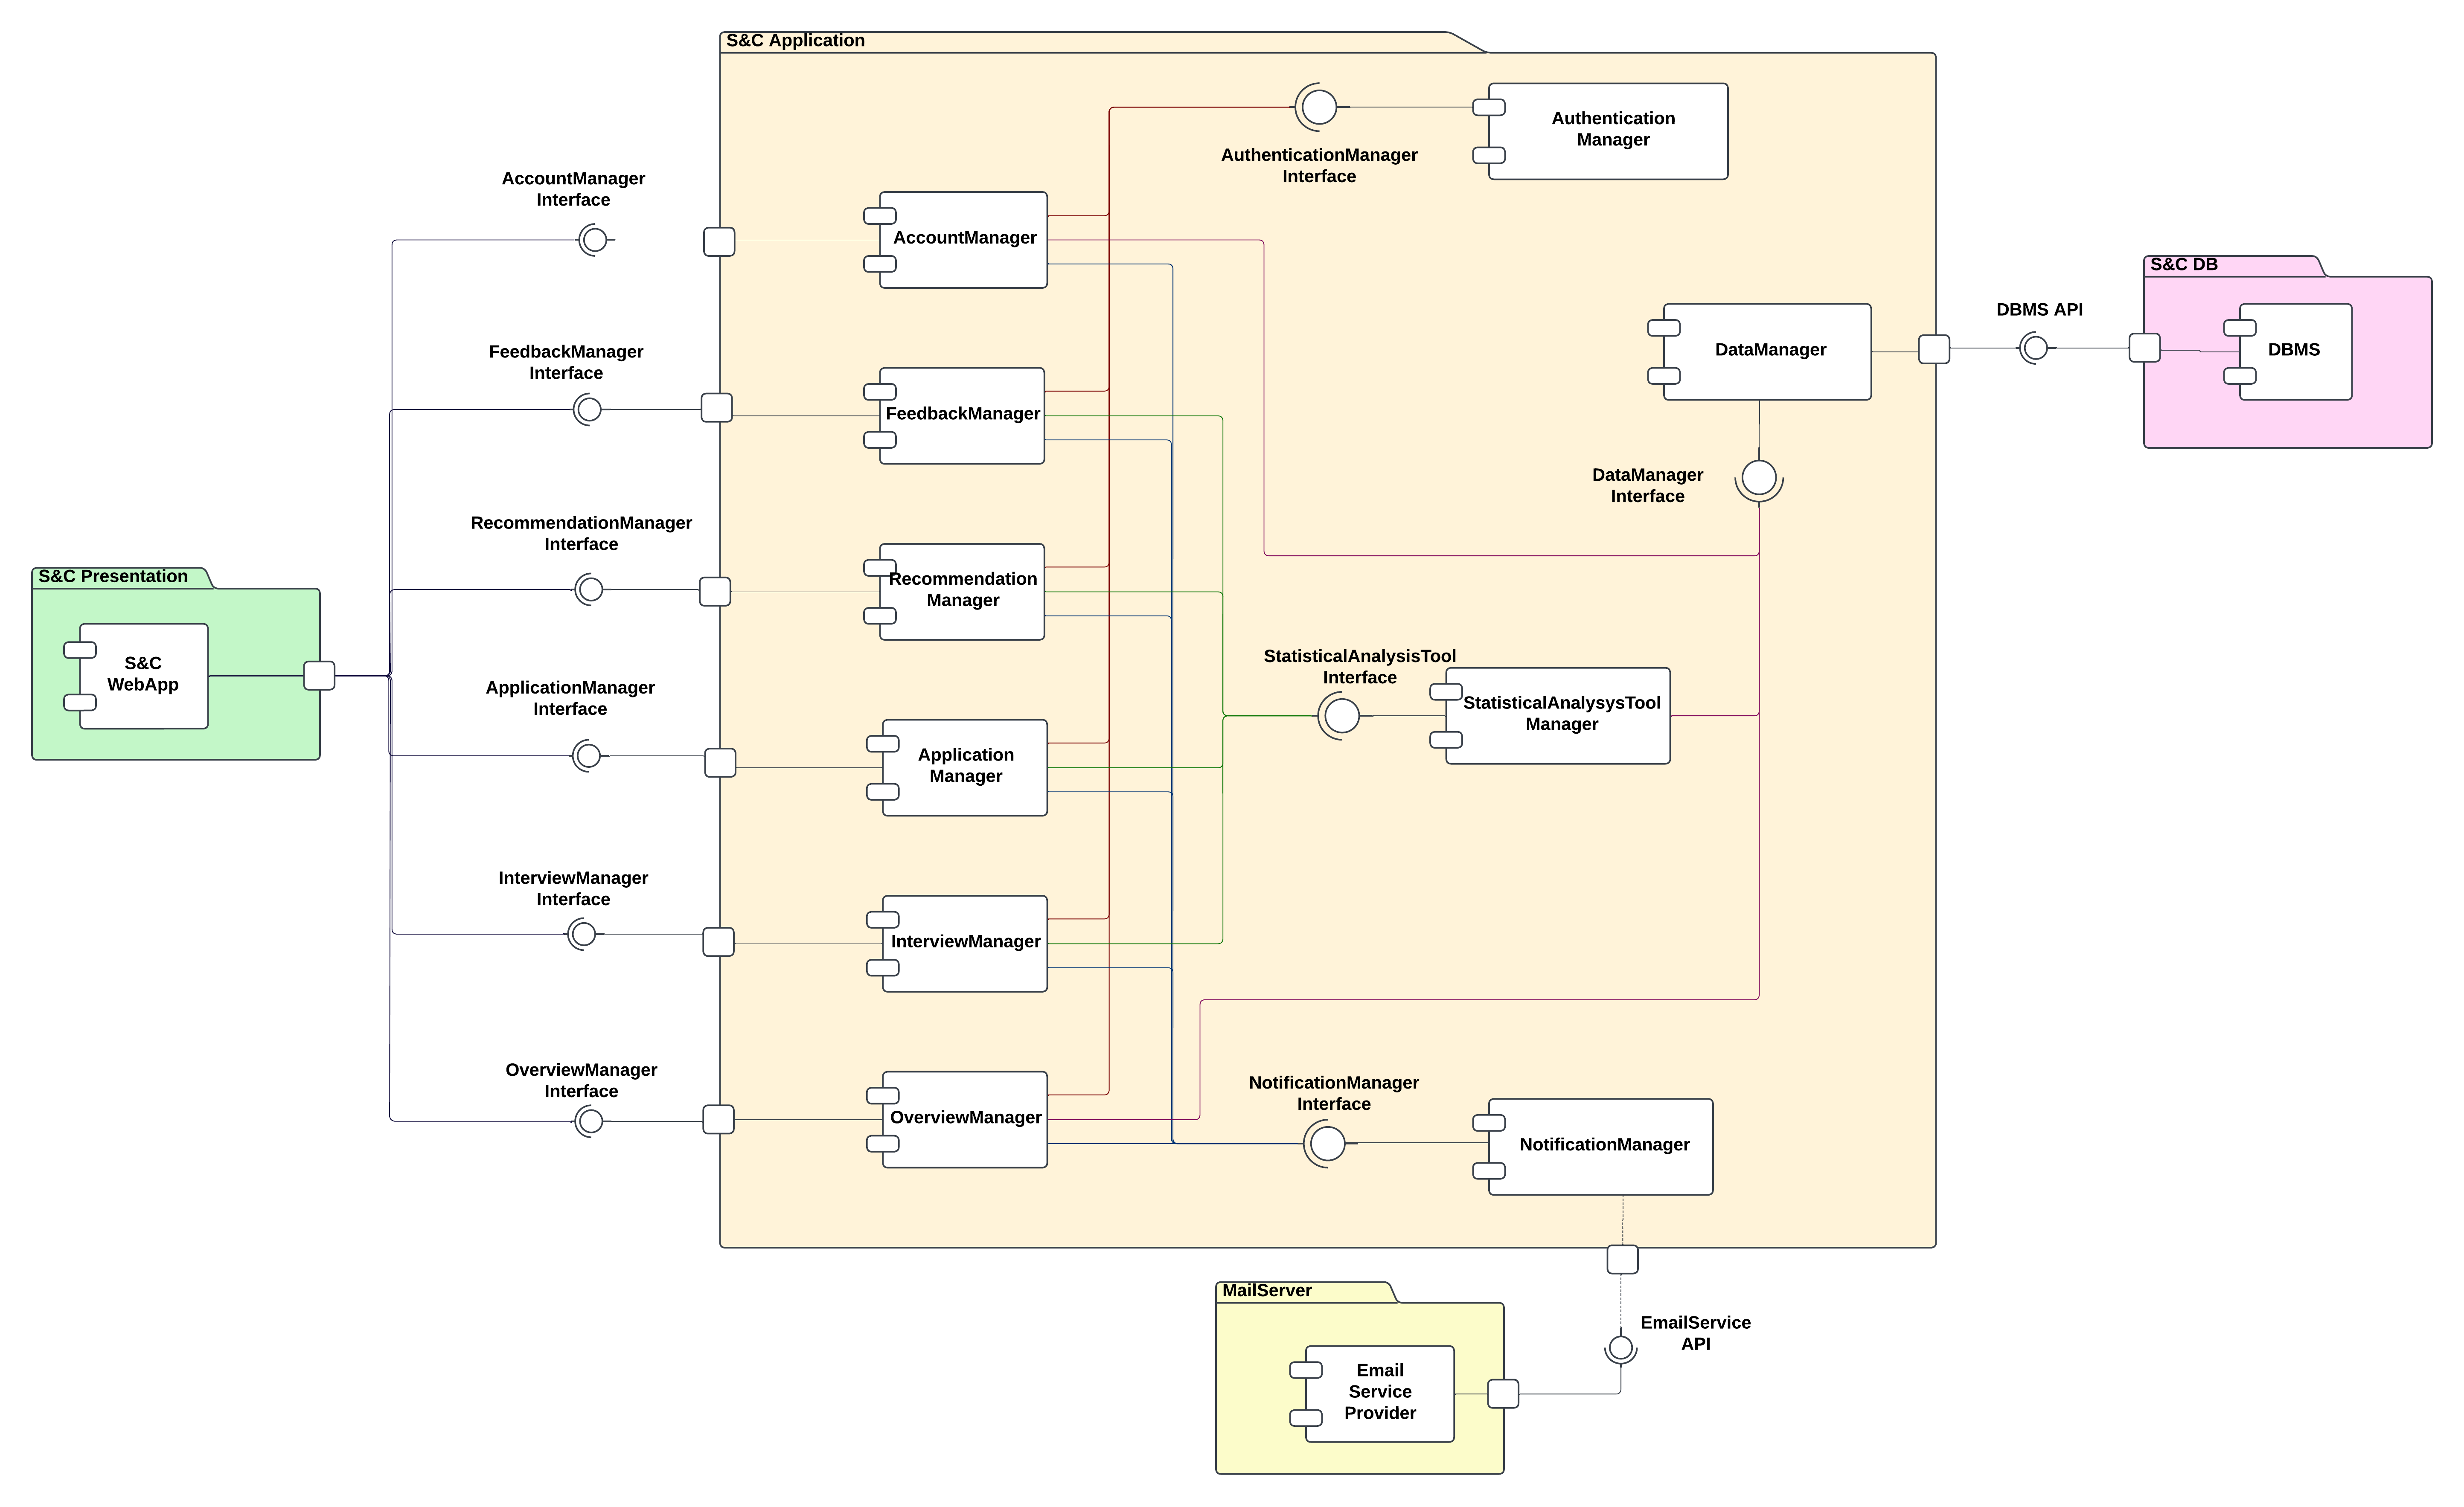
\includegraphics[width=1.1\linewidth]{DD//Images/ComponentDiagram.png}
    \caption{Component Diagram }
\end{figure}



\begin{itemize}
    \item \textbf{WebApp:} The WebApp serves as the primary interface for all users: students, companies, and universities, allowing them to interact with the application via their web browser. User requests are processed and sent to the appropriate backend components through the defined interfaces.
    \item \textbf{Account Manager:} The Account Manager is a backend module responsible for managing all aspects of account registration, login, and user data. It handles the creation of different user profiles and ensures the validity of the submitted data. The Account Manager communicates with the Notification Manager to send notifications to users as needed. To save the new user's data, the Account Manager interacts with the Data Manager to store the information in the database. However, before performing any database operations, the Account Manager first requests permission from the Authentication Manager to ensure that the user is authenticated and authorized to perform the action.
    \item \textbf{Feedback Manager:} The Feedback Manager is responsible for gathering user feedback from both students and companies. It proactively requests feedback when needed through the Notification Manager, ensuring user engagement. This module collaborates with the Statistical Analysis Tool by providing updated feedback data, enabling continuous improvement of the recommendation system and analysis capabilities.
    \item \textbf{Recommendation Manager:} The Recommendation Manager is the module that is responsible for requesting and receiving internship matches between students and projects from the Statistical Analysis Tool. After obtaining the matches, it communicates the results to the Notification Manager, which then notifies the involved users about the recommended opportunities.
    \item \textbf{Application Manager:} The Application Manager handles student applications in three scenarios: when a student proactively applies for an internship they are interested in when a student accepts a recommendation, and when he responds to an invitation from a company that has previously accepted the system's recommendation. After processing the applications, it communicates with the Notification Manager to notify both students and companies about the submitted applications. Additionally, it interacts with the Statistical Analysis Tool to provide data for further analysis and improvement of the recommendation system.
    \pagebreak
    \item \textbf{Interview Manager:} The Interview Manager oversees the entire interview and final selection process. It communicates with the Notification Manager to keep both students and companies informed about new developments throughout the process. Additionally, it interacts with the Statistical Analysis Tool to provide data, such as information on who was selected for the job, helping to refine the system and adjust parameters for future job recommendations.
    \item \textbf{Overview Manager:} The Overview Manager is responsible for monitoring ongoing internships. It communicates with the Notification Manager to keep universities, students, and companies involved in the project updated on progress. Additionally, it interacts with the Authentication Manager to obtain permission for accessing data and then works with the Data Manager to insert and register the relevant updates.
    \item \textbf{StatisticalAnalysisTool Manager:} The Statistical Analysis Tool Manager is responsible for generating matches between students and internship projects based on student CVs and project descriptions. It also provides suggestions to students for improving their CVs and to companies for enhancing their project descriptions. These tasks are performed using a recommendation system powered by AI and machine learning. The tool is continuously refined through feedback from both students and companies about its previous recommendations. It communicates with the Data Manager to access the necessary data, with prior authentication provided by the Authentication Server.
    \item \textbf{Notification Manager:} The Notification Manager is responsible for sending notifications to all users across various channels. It interacts with the email service API to send email notifications and also delivers real-time updates directly within the web app. When delivering notifications through the app, it follows the chain of requests, processing them in reverse order to ensure that all relevant parties receive the appropriate updates.
    \item \textbf{Authentication Manager:} The Authentication Manager is responsible for managing access rights to data, ensuring that users can perform read or write operations based on their role and permissions.
    \item \textbf{Data Manager:} The Data Manager is responsible for managing and storing all data within the system. It handles data retrieval, updates, and ensures that information is accurately recorded and stored. The module interacts with other components to provide the necessary data for operations while maintaining data integrity and security.
    \item \textbf{Email Service Provider:} The Email Service Provider is an external module that interacts with the Notification Manager to send email notifications to users. It handles the delivery of emails for various events, such as application updates, interview schedules, and system alerts.
    \item \textbf{DBMS:} The DBMS (Database Management System) is responsible for managing and organizing the system's database. It handles data storage, retrieval, and manipulation, ensuring data integrity, security, and efficient access. The DBMS interacts with other modules to support operations such as user authentication, data analysis, and application management, storing and managing all relevant information within the system.
    
\end{itemize}

\pagebreak
\section{Deployment view}
\begin{figure}[H]
    \centering
    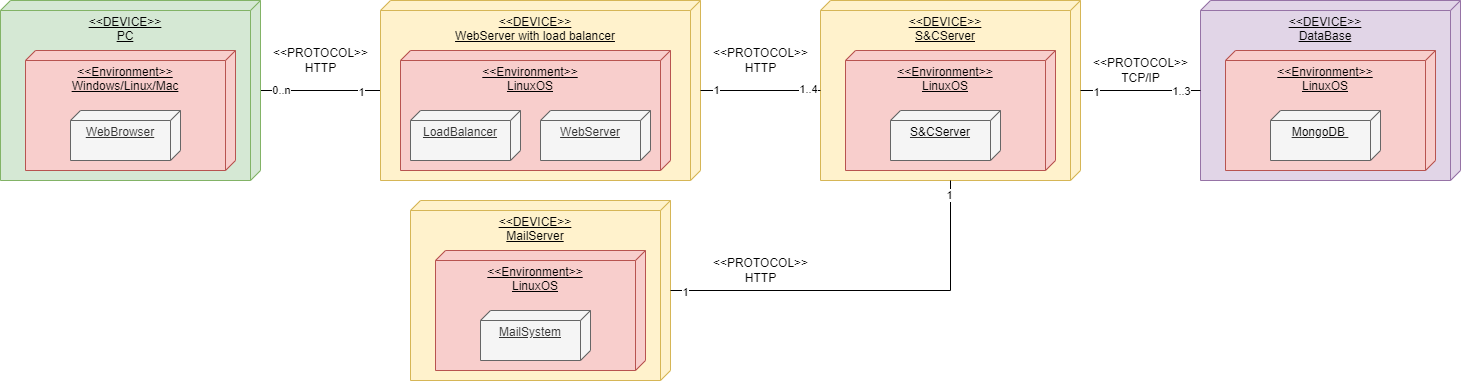
\includegraphics[width=1\linewidth]{DD//Images/deployment.drawio.png}
    \caption{Deployment view}
    \label{fig:enter-label}
\end{figure}

The deployment view illustrates how the Students \& Companies system components are distributed across various nodes. Users interact with the platform through a Web Browser running on a client device (Windows, Linux, or MacOS), which communicates with the Web Server over HTTPS. The Web Server includes a Load Balancer to efficiently distribute requests among multiple backend services, ensuring scalability and reliable performance under varying traffic loads.

The Application Server, deployed on a Linux environment, handles core application logic, hosting the managers responsible for user accounts, recommendations, feedback, and other functionalities. The Mail Server, running on a separate Linux node, manages email notifications, ensuring communication between the platform and its users. Data storage and retrieval are managed by the Database Server, powered by MongoDB on a Linux environment, which interacts with the application layer over TCP/IP. This setup ensures a clear separation of responsibilities, allowing for modular development and easy scalability.

\pagebreak
\section{Runtime view}

All the sequence diagrams described in the Requirements Analysis and Specification Document (RASD) will be elaborated in greater detail. In this expanded version, we will identify and specify the individual components of the application that are utilized to fulfill each specific functionality. 

Here below we will include a visual example (sequence diagrams) of how each application component contributes to the implementation of the corresponding functionality. By doing so, we hope to provide a clearer understanding of the interaction between various components and their roles in achieving the described features and requirements.

Note on the sequence diagram: we did not model calls to the DBMS, since every time the DataManager is called it handles them all in the same way with the methods we will show in the next chapter.

\textbf{UC1: Student creates an account}

This sequence diagram outlines the student registration process in the web app. It covers data submission, duplicate account checks, email verification, and optional CV upload. Notifications are handled via email, and validated accounts are saved in the database. Once the CV has been uploaded some calls are made to the statisticalAnalysisTool, but their return, the improvement suggestions and the matches, is not modeled since it will be handled in other use cases.

%\begin{figure}[H]
   % \centering
    %\includegraphics[width=1\linewidth]%{DD//Images/SequenceDiagrams/UC1.png}
    %\caption{UC1}
%\end{figure}


\begin{figure}[H]
    \centering
    %\hspace{-3cm} % Adjust this value as needed to move the image lef
    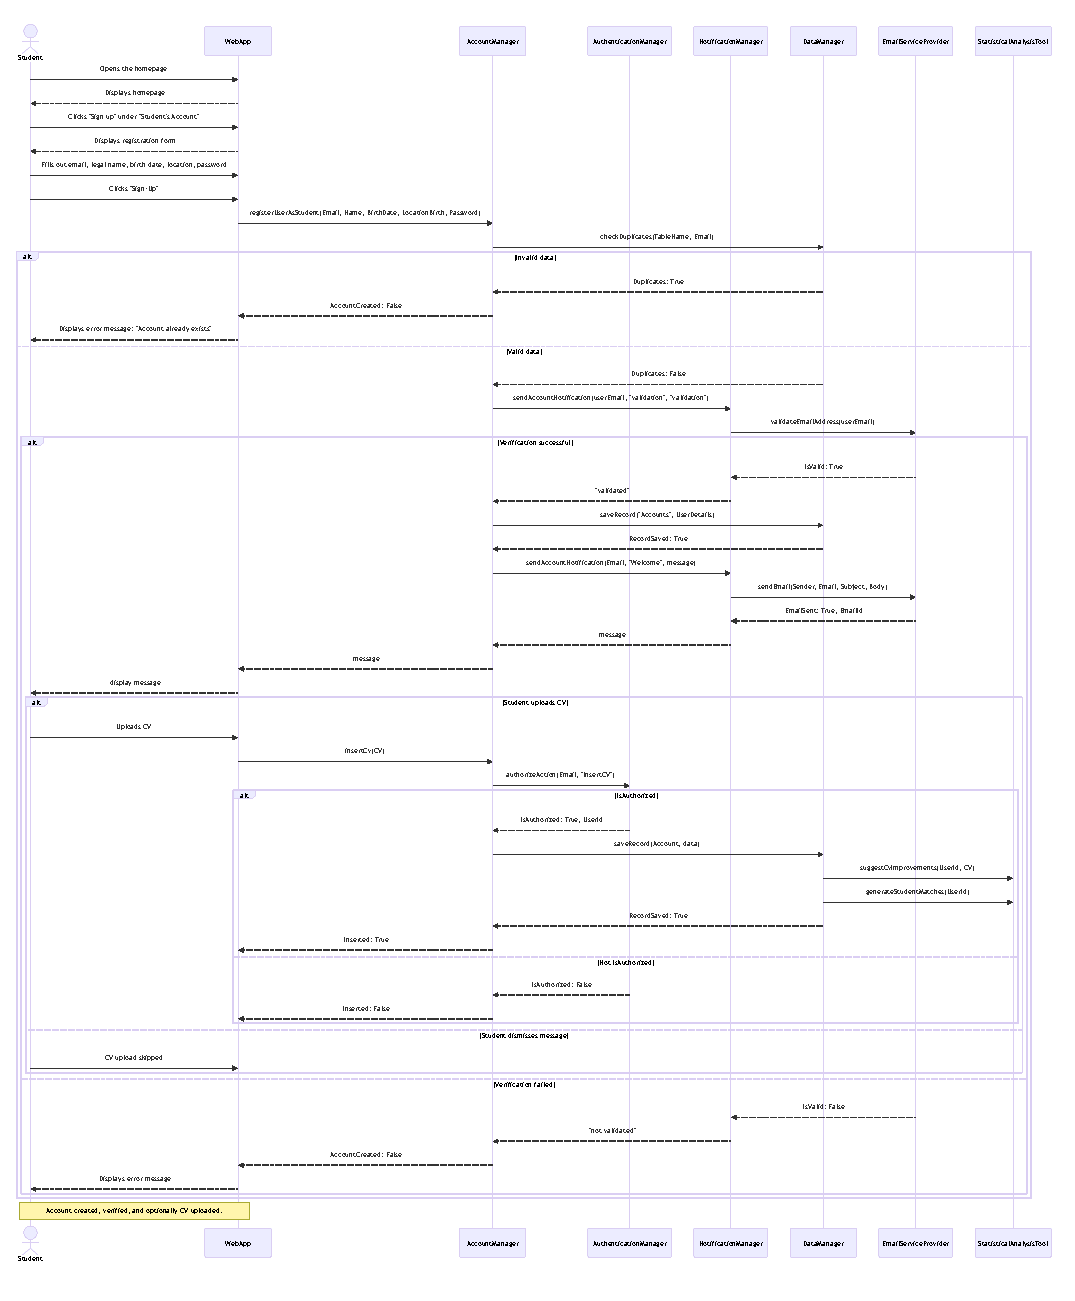
\includegraphics[width=1.1\linewidth]{DD//Images/SequenceDiagrams/UC1.pdf}
    \caption{UC1}
\end{figure}

\newpage
\textbf{UC2: Company creates an account}

This sequence diagram outlines the company registration process in the web app. It includes data submission, duplicate account checks, email verification, and project description upload. Notifications are managed via email, and validated accounts are stored in the database. Once the project description has been uploaded some calls are made to the statisticalAnalysisTool, but their return, the improvement suggestions and the matches, is not modeled since it will be handled in other use cases.


%\begin{figure}[H]
  %  \centering
   % \includegraphics[width=1\linewidth]%{DD//Images/SequenceDiagrams/UC2.png}
  %  \caption{UC2}
%\end{figure}

\begin{figure}[H]
    \centering
    %\hspace{-1cm} % Adjust this value as needed to move the image lef
    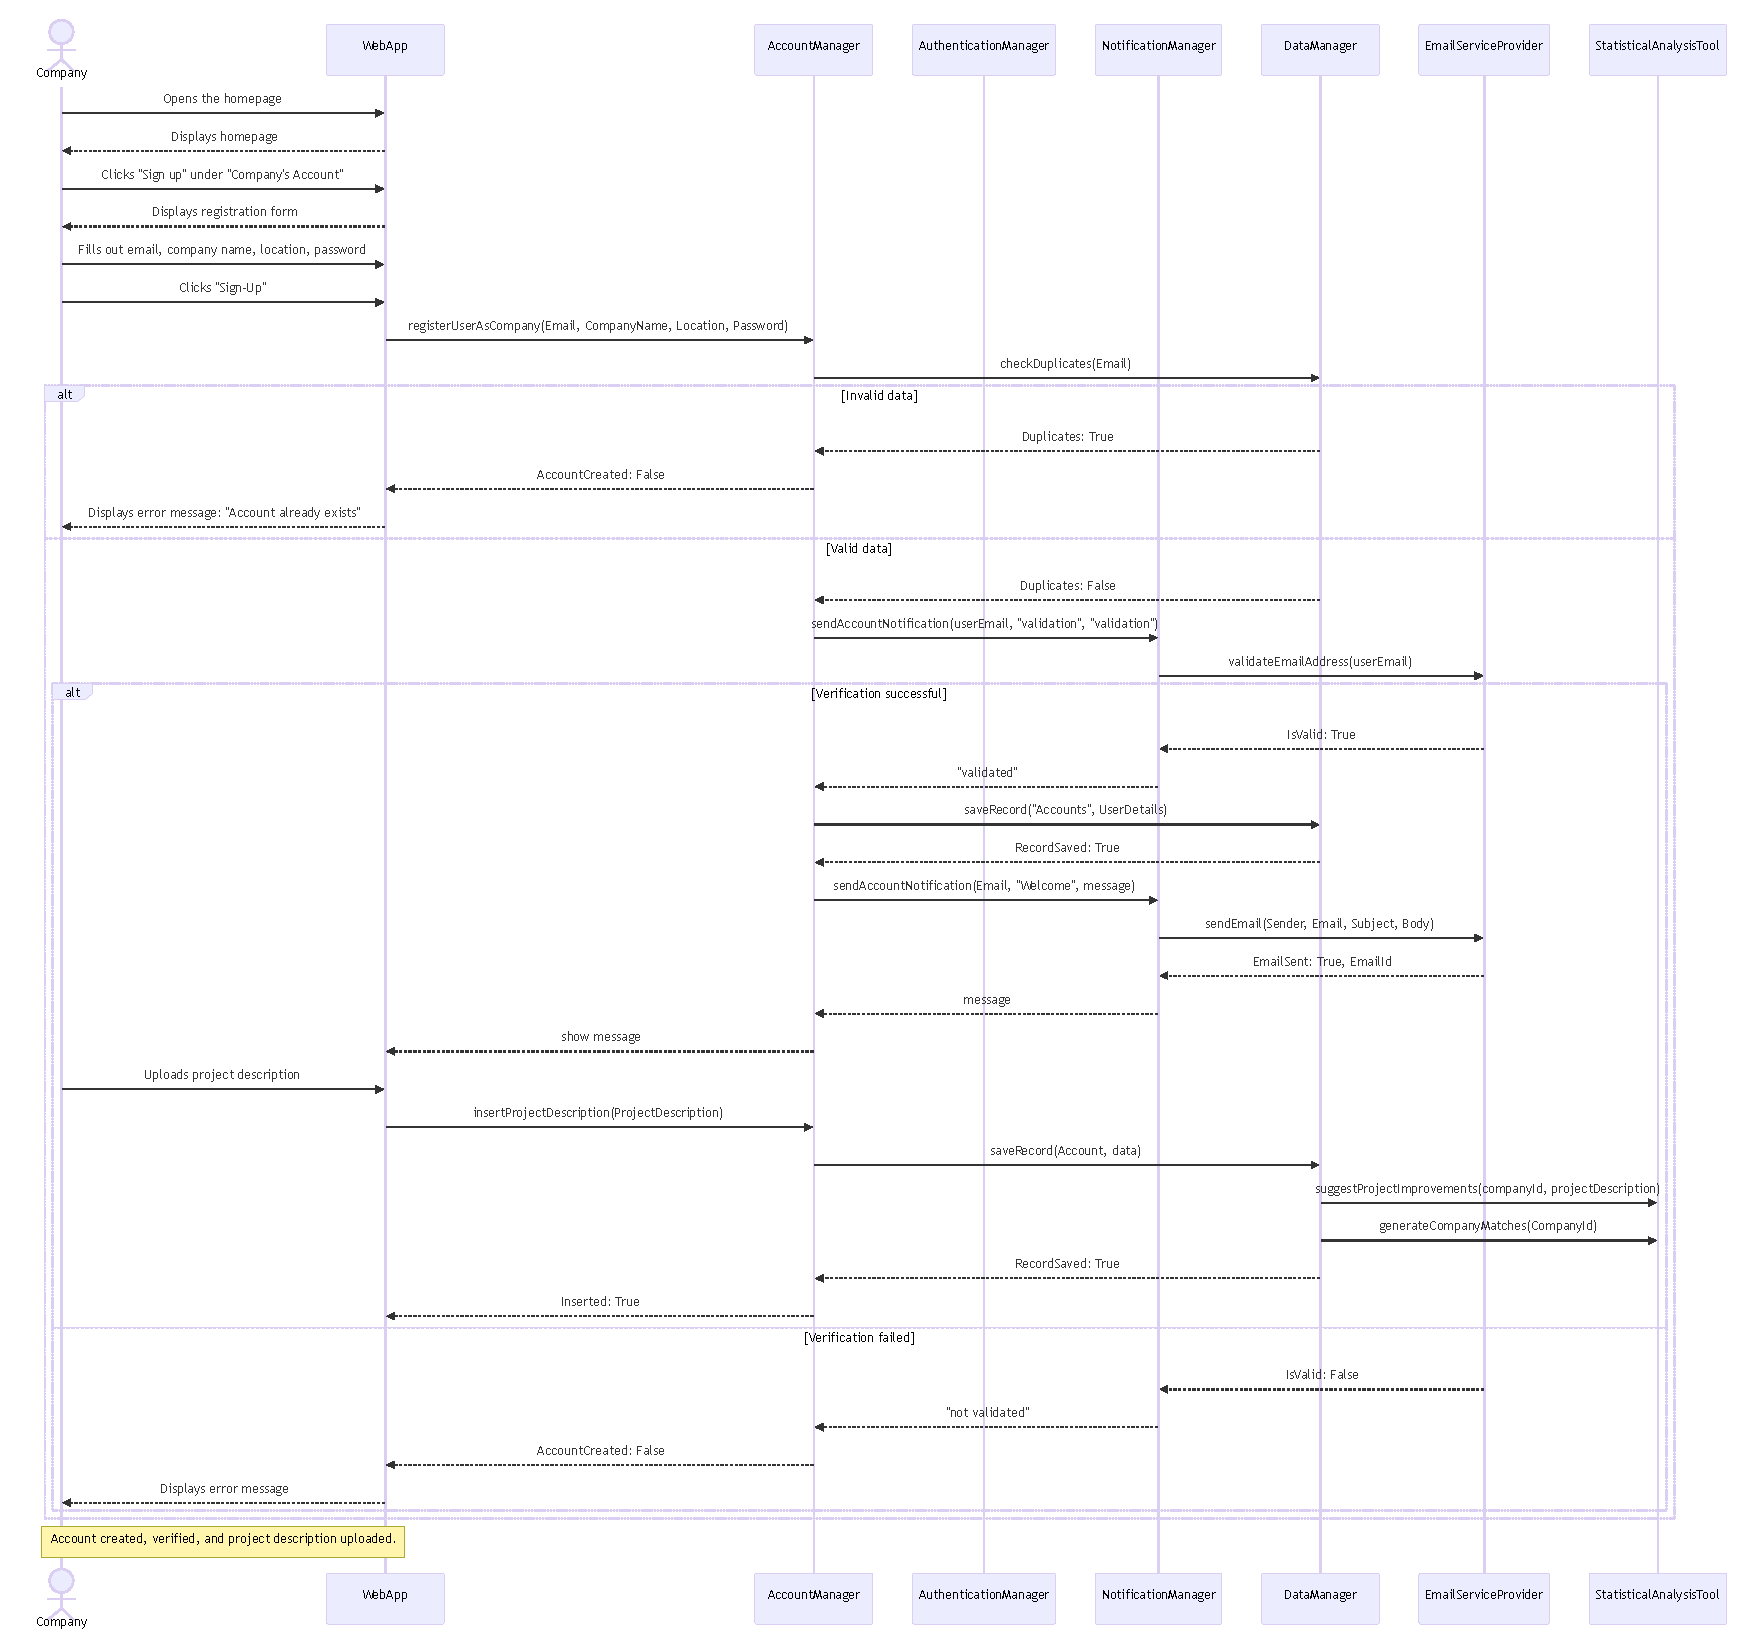
\includegraphics[width=1.1\linewidth]{DD//Images/SequenceDiagrams/UC2}
    \caption{UC2}
\end{figure}

\newpage
\textbf{UC3: Student searches and applies for an internship}

This sequence diagram describes the internship application process for students in the web app. It includes navigation to the global page, viewing internship details, and applying if interested. Successful applications trigger data updates in the system and notifications to companies via email. If the student is not interested, they return to the global page. 

\begin{figure}[H]
    \centering
    %\hspace{-3cm} % Adjust this value as needed to move the image lef
    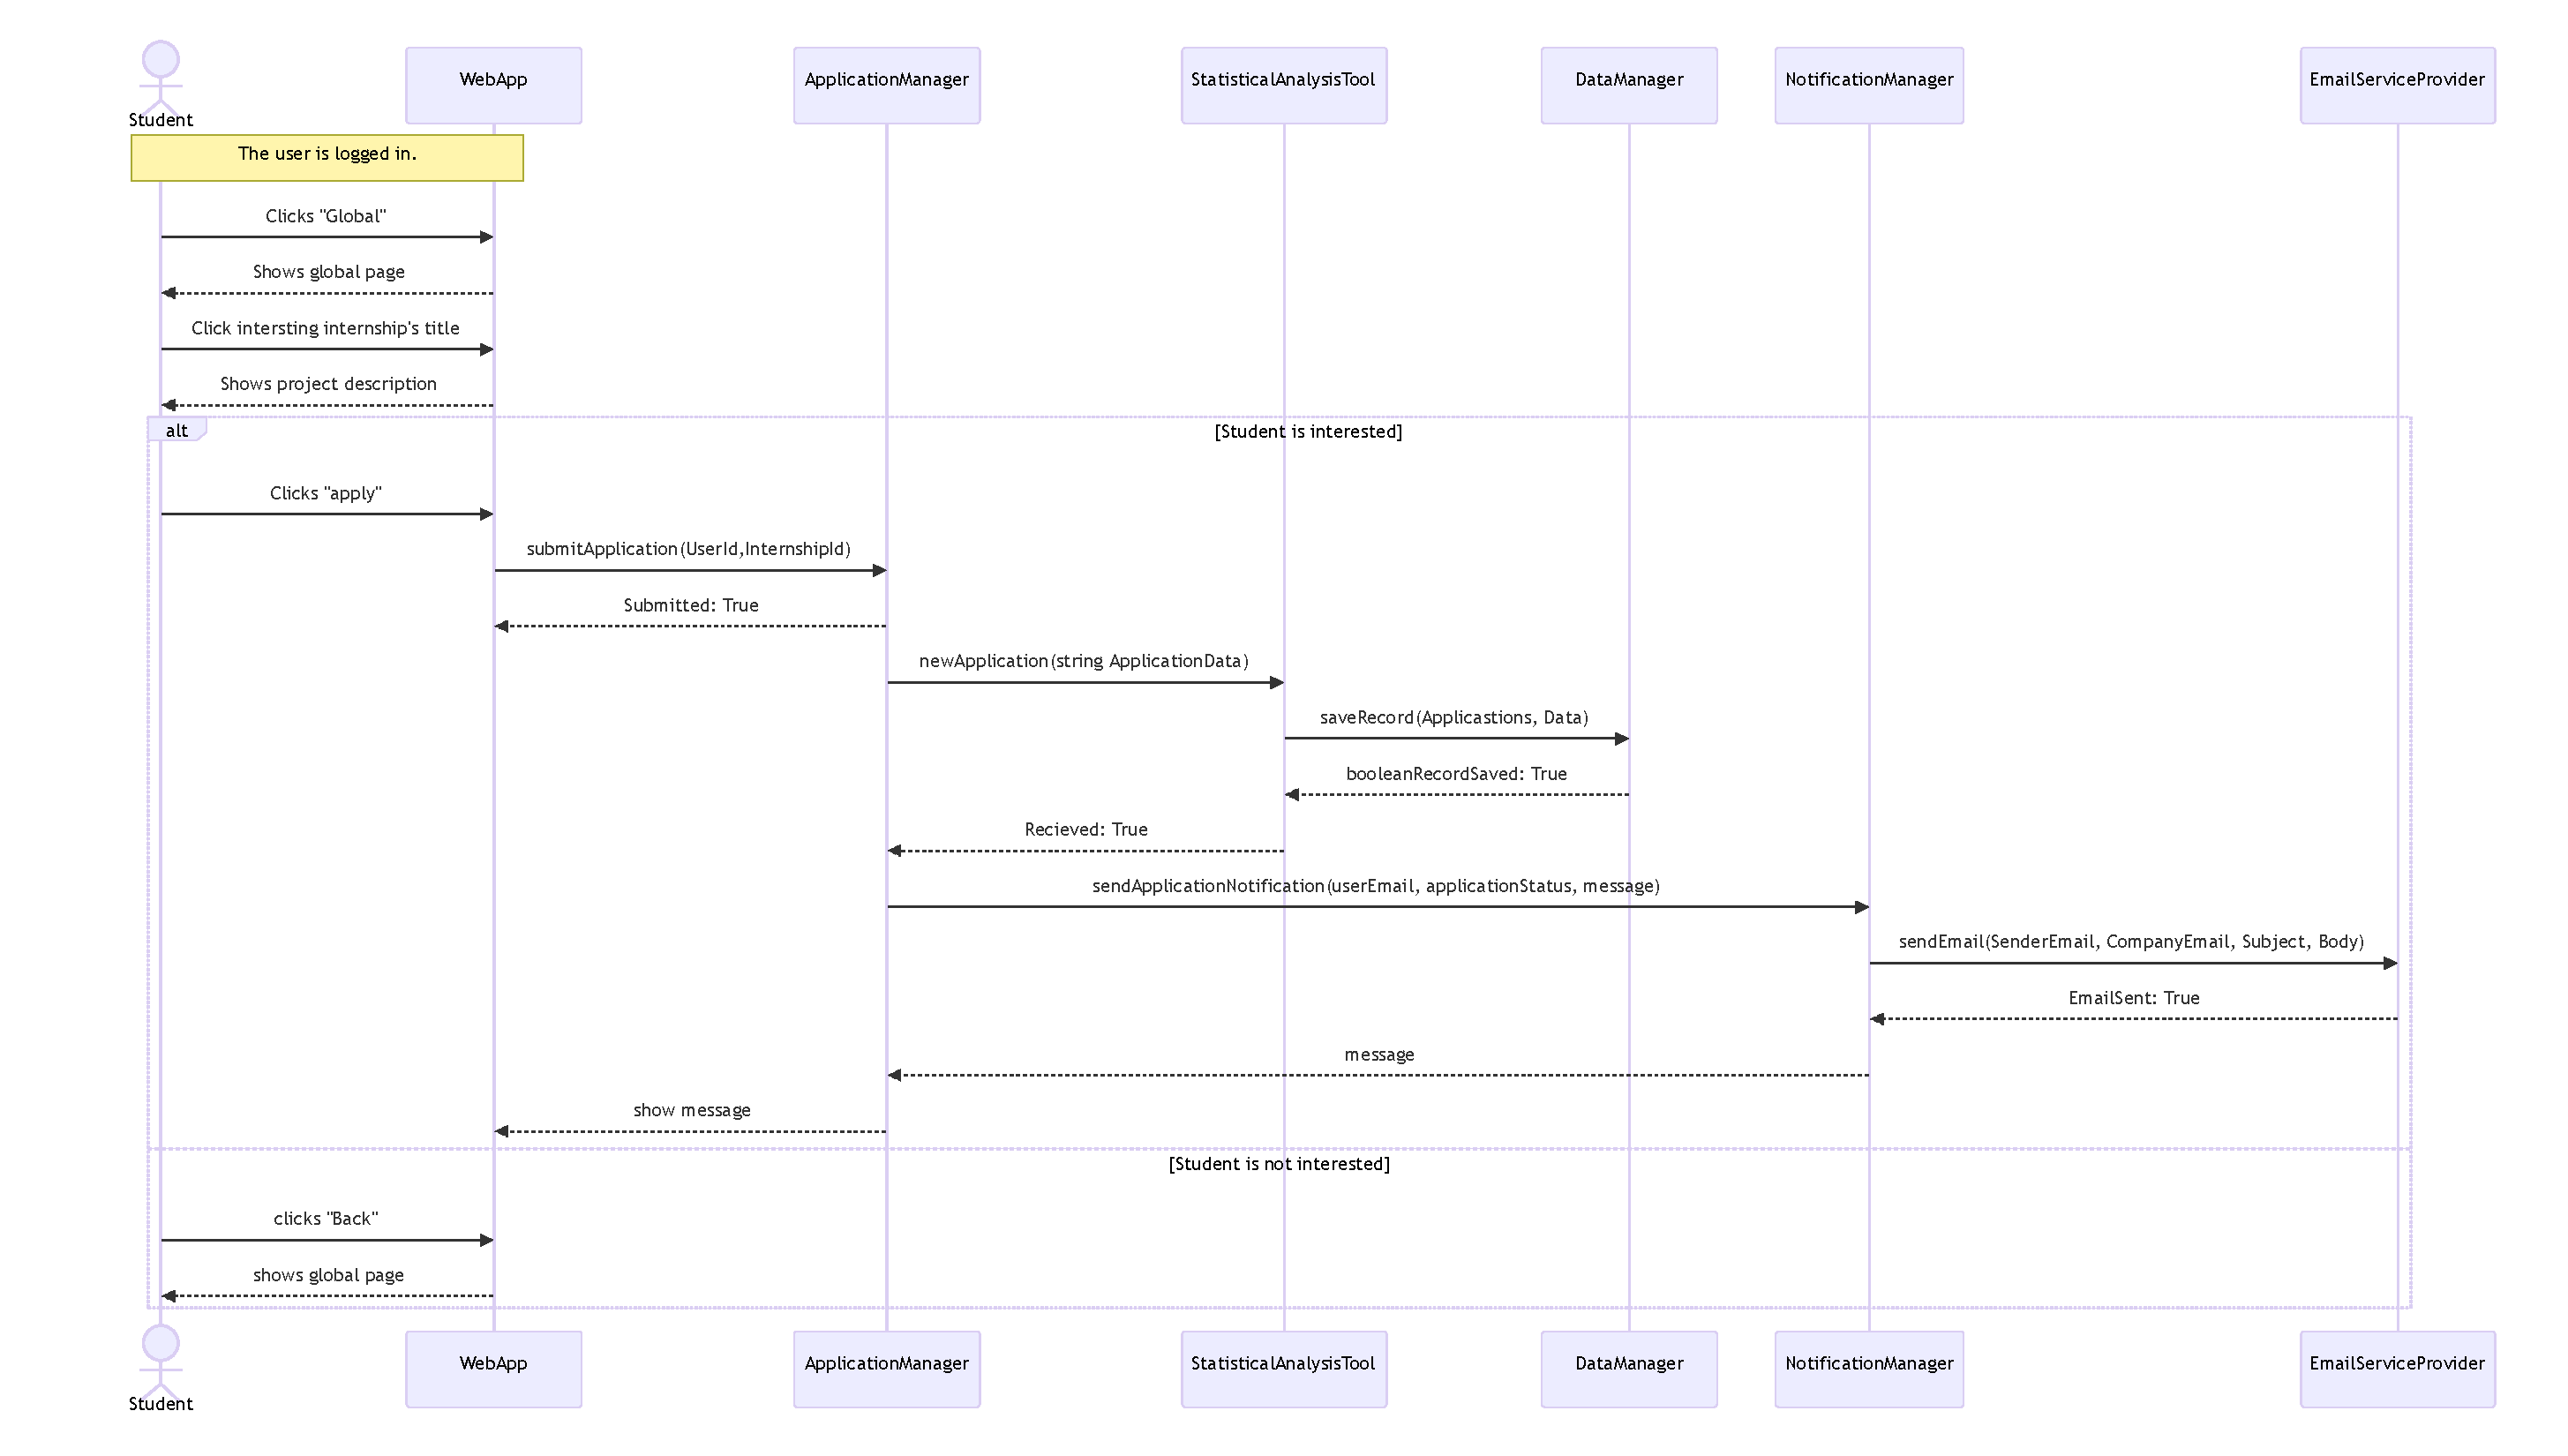
\includegraphics[width=1.1\linewidth]{DD//Images/SequenceDiagrams/UC3.pdf}
    \caption{UC3}
\end{figure}

\newpage
\textbf{UC4: Student recieves an internship recommendation}

This sequence diagram illustrates the recommendation handling process for students in a web app. Recommendations are generated by the StatisticalAnalysisTool, notified to the student via email, and displayed in the app. The display of this notification is modeled as a message call to the WebApp, this is due to the fact that we chose to model all calls to the WebApp that show a notification using the word: message (a convention also applied in future diagrams); the arrow is not dotted since here this message call is not directly a return of another one, but it starts from the RecommendationManager. Students can either accept the recommendation by applying for the internship, which updates the system and notifies the company, or reject it, which removes the match and informs the company of the rejection.

\begin{figure}[H]
    \centering
    %\hspace{-1cm} % Adjust this value as needed to move the image lef
    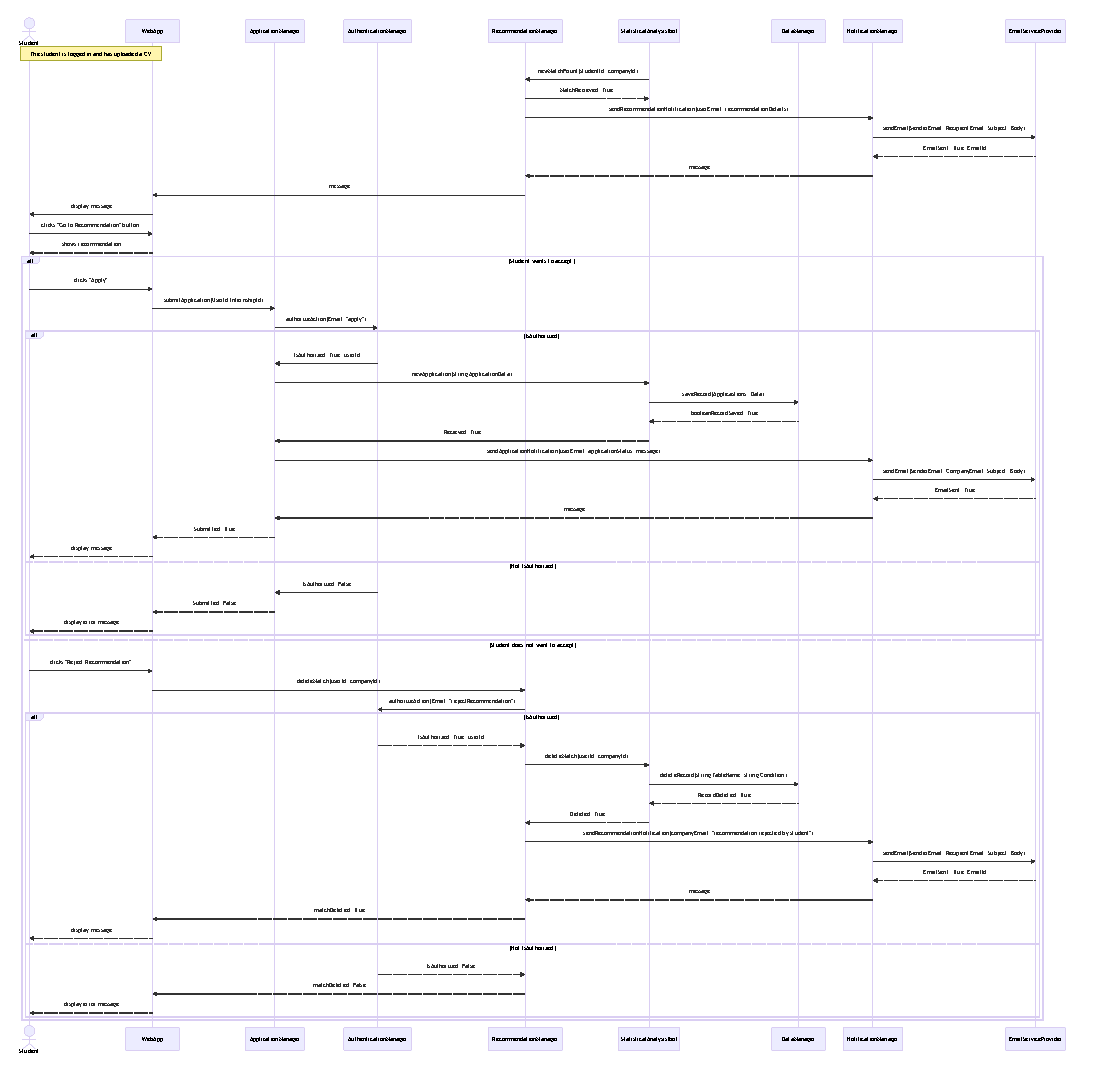
\includegraphics[width=1.1\linewidth]{DD//Images/SequenceDiagrams/UC4.pdf}
    \caption{UC4}
\end{figure}

\newpage
\textbf{UC5: Company recieves a student's recommendation}

This sequence diagram illustrates the recommendation handling process for companies in a web app. After logging in and uploading a project description, companies are notified of student matches generated by the StatisticalAnalysisTool via email and app notifications (same procedure described in the previous diagram's description). Companies can choose to accept or reject the recommendations. If they are interested in a student, and the student has already applied, the company accepts the application and notifies the student. If the student hasn’t applied, the company invites the student to apply. If the company isn’t interested, and the student has applied, the application is rejected, and the student is notified. If the student hasn’t applied, the company rejects the recommendation, removes the match, and notifies the student.
\begin{figure}[H]
    \centering
    \hspace{-1 cm} % Adjust this value as needed to move the image left
    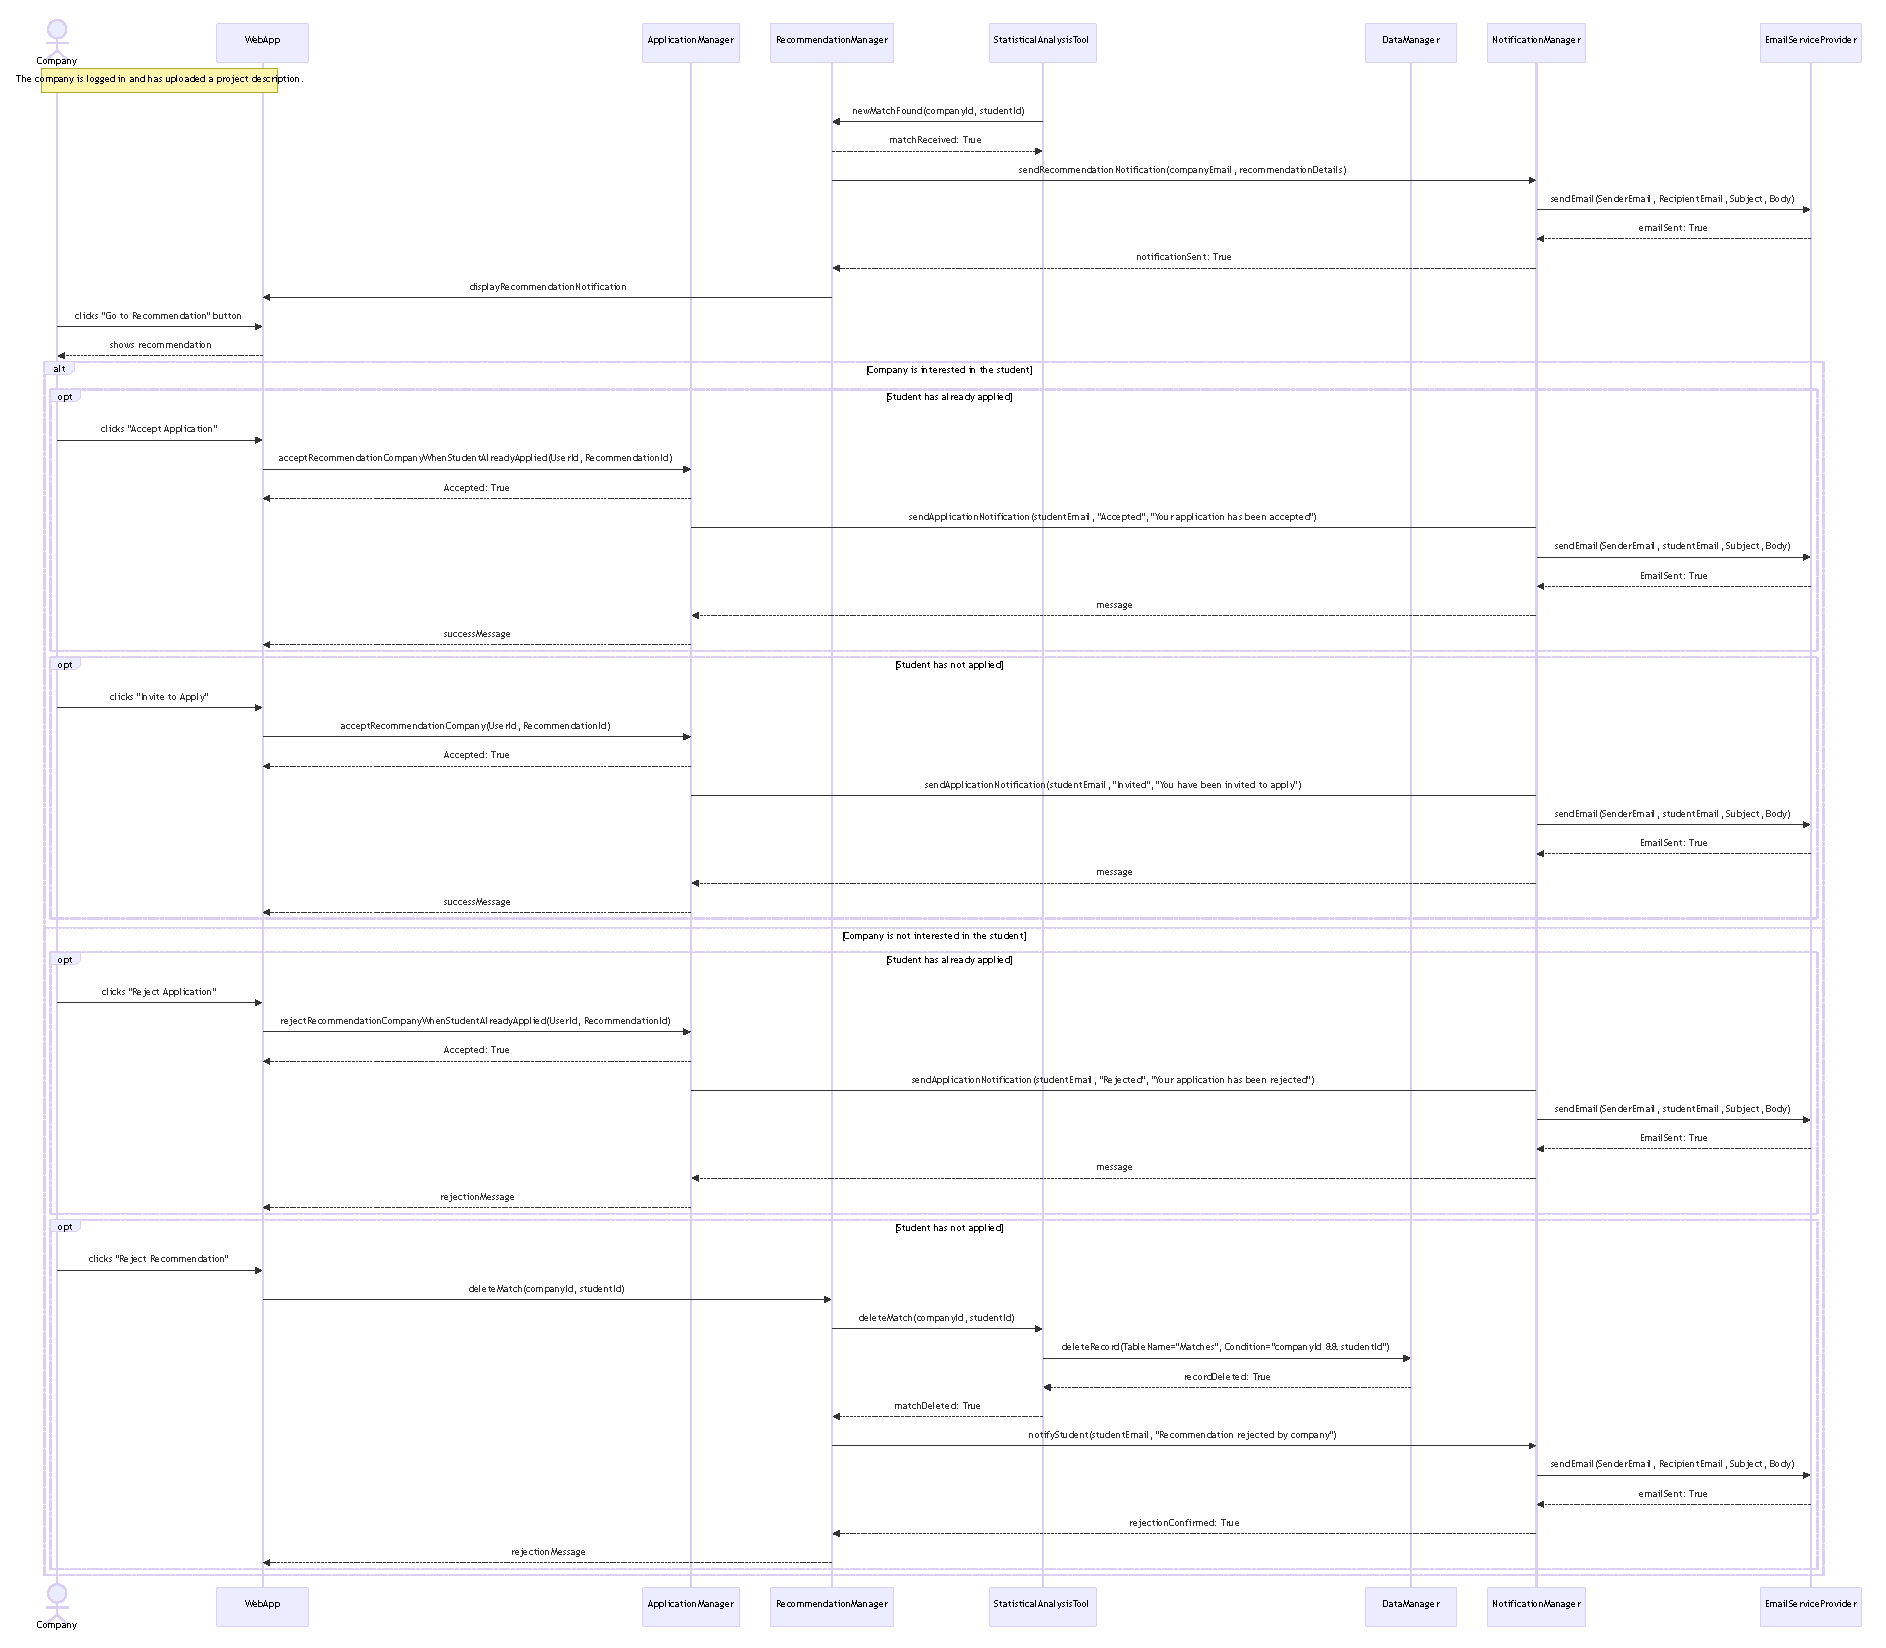
\includegraphics[width=1\linewidth]{DD//Images/SequenceDiagrams/UC5.pdf}
    \caption{UC5}
\end{figure}

\newpage
\textbf{UC6: Interview}

This sequence diagram illustrates a simplified version of the interview use case. We chose to do a simplified sequence diagram denoting only the basic flow of events, since otherwise it would have been very big and unreadable. The flow of events described is the case in which the university initiates contact, and the system notifies the student of it; then the university creates an assessment, and evaluates it after the student has responded (we did not model the student's action of filling the assessment). The student is then selected and the company schedules the interview using the system.

\begin{figure}[H]
    \centering
    \hspace{-1 cm} % Adjust this value as needed to move the image left
    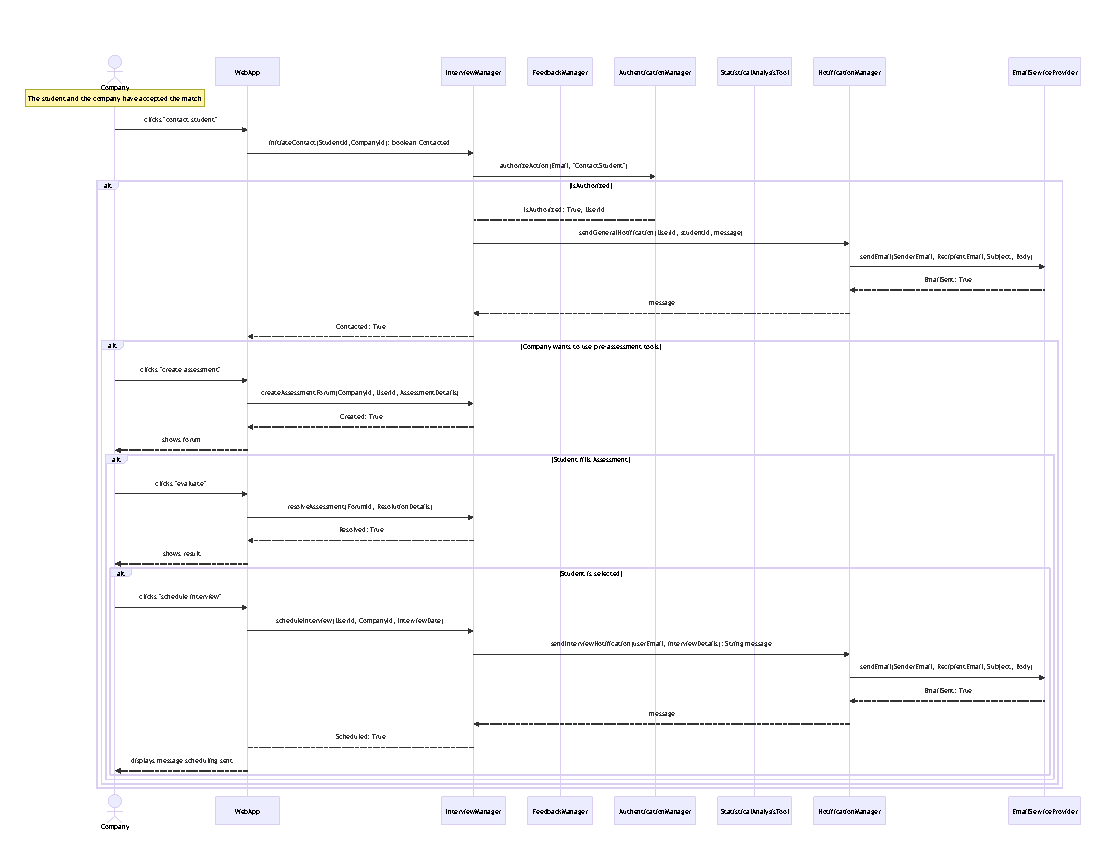
\includegraphics[width=1.1\linewidth]{DD//Images/SequenceDiagrams/UC6.pdf}
    \caption{UC6}
\end{figure}

\newpage
\textbf{UC7: User leaves feedback}

This sequence diagram illustrates the process of leaving internship feedback in the web app. After the user participates in an internship, they receive a feedback notification via email. If the user decides to leave feedback, they fill out a form, which triggers an authorization check. If authorized, the feedback is submitted, saved in the database, and confirmed in the web app. If not authorized, the submission is rejected. If the user chooses not to leave feedback, the message is simply closed without any action.

\begin{figure}[H]
    \centering
    \hspace{-1 cm} % Adjust this value as needed to move the image left
    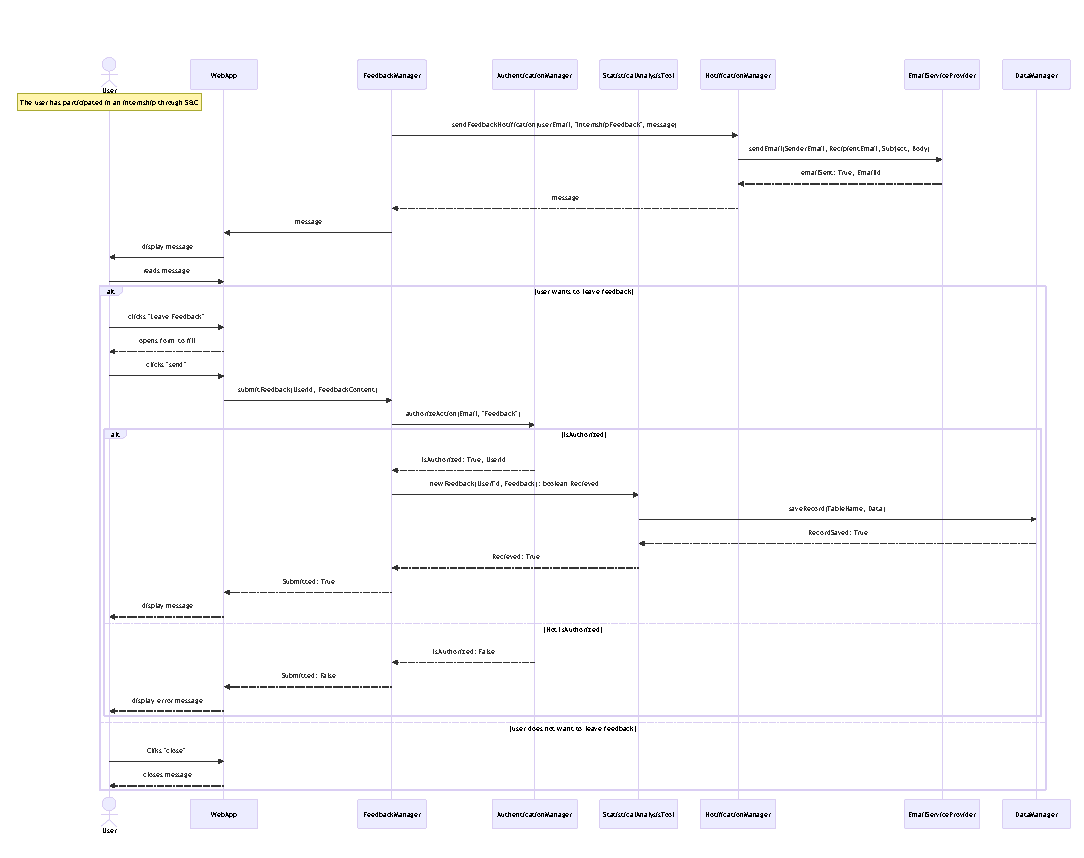
\includegraphics[width=1.1\linewidth]{DD//Images/SequenceDiagrams/UC7.pdf}
    \caption{UC7}
\end{figure}

\newpage
\textbf{UC8: Student recieves suggestion on CV}

This sequence diagram describes the process of CV improvement suggestions for a student. After the student uploads their CV, the StatisticalAnalysisTool generates improvement suggestions and sends a notification via email through the NotificationManager and EmailServiceProvider. The suggestion is then displayed on the web app (as previously described). If the student finds the suggestion useful, they can upload a new version of the CV, which triggers an authorization check through the AuthenticationManager. If authorized, the CV is updated, and the suggestion process continues by calling the statisticalAnalysisTool (the return is not shown since it would be a loop of this use case). If the student doesn’t find the suggestion useful, they can close it, and no changes are made to the system.

\begin{figure}[H]
    \centering
    \hspace{-1 cm} % Adjust this value as needed to move the image left
    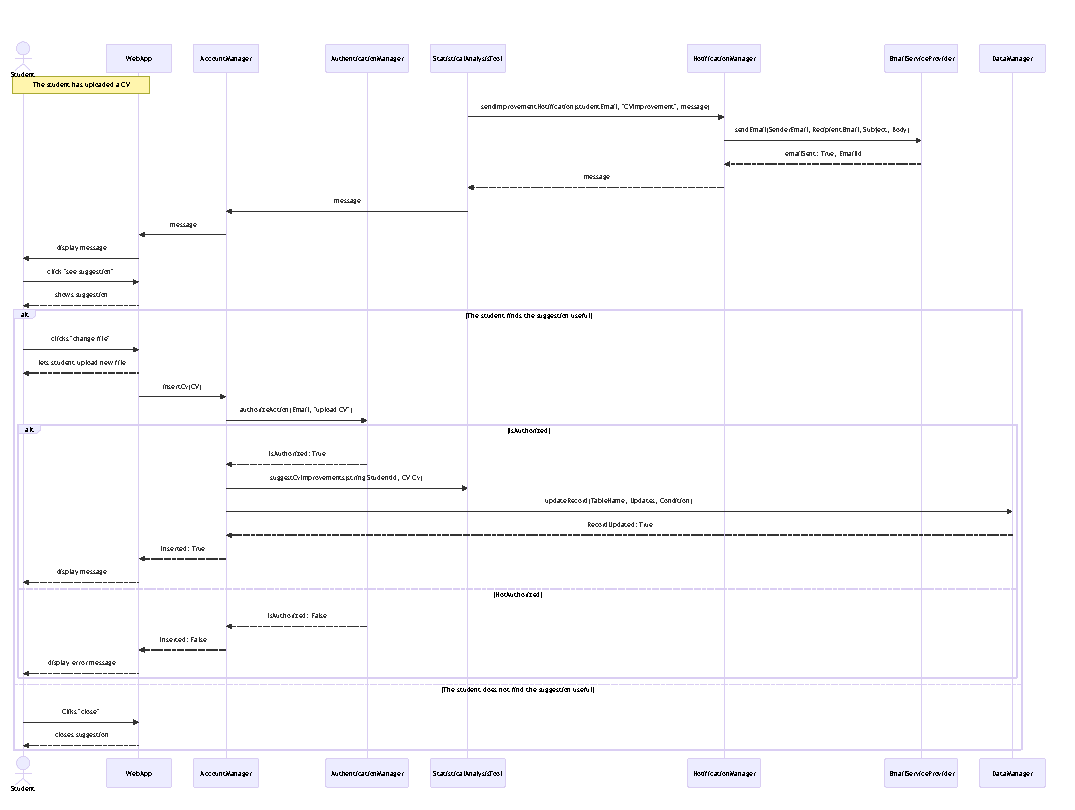
\includegraphics[width=1.1\linewidth]{DD//Images/SequenceDiagrams/UC8.pdf}
    \caption{UC8}
\end{figure}

\newpage
\textbf{UC9: Company recieves suggestion on project description}

This sequence diagram describes the process for a company to handle project description improvement suggestions the web app. After uploading a project description, the company receives a suggestion via email. If the company finds the suggestion useful, they can modify the project description, triggering an authorization check. If authorized, the description is updated, the changes are saved in the database and the statisticalAnalysisTool is notified. If not authorized, the modification is rejected. If the company does not find the suggestion useful, they can simply close the suggestion without making any changes.

\begin{figure}[H]
    \centering
    \hspace{-1 cm} % Adjust this value as needed to move the image left
    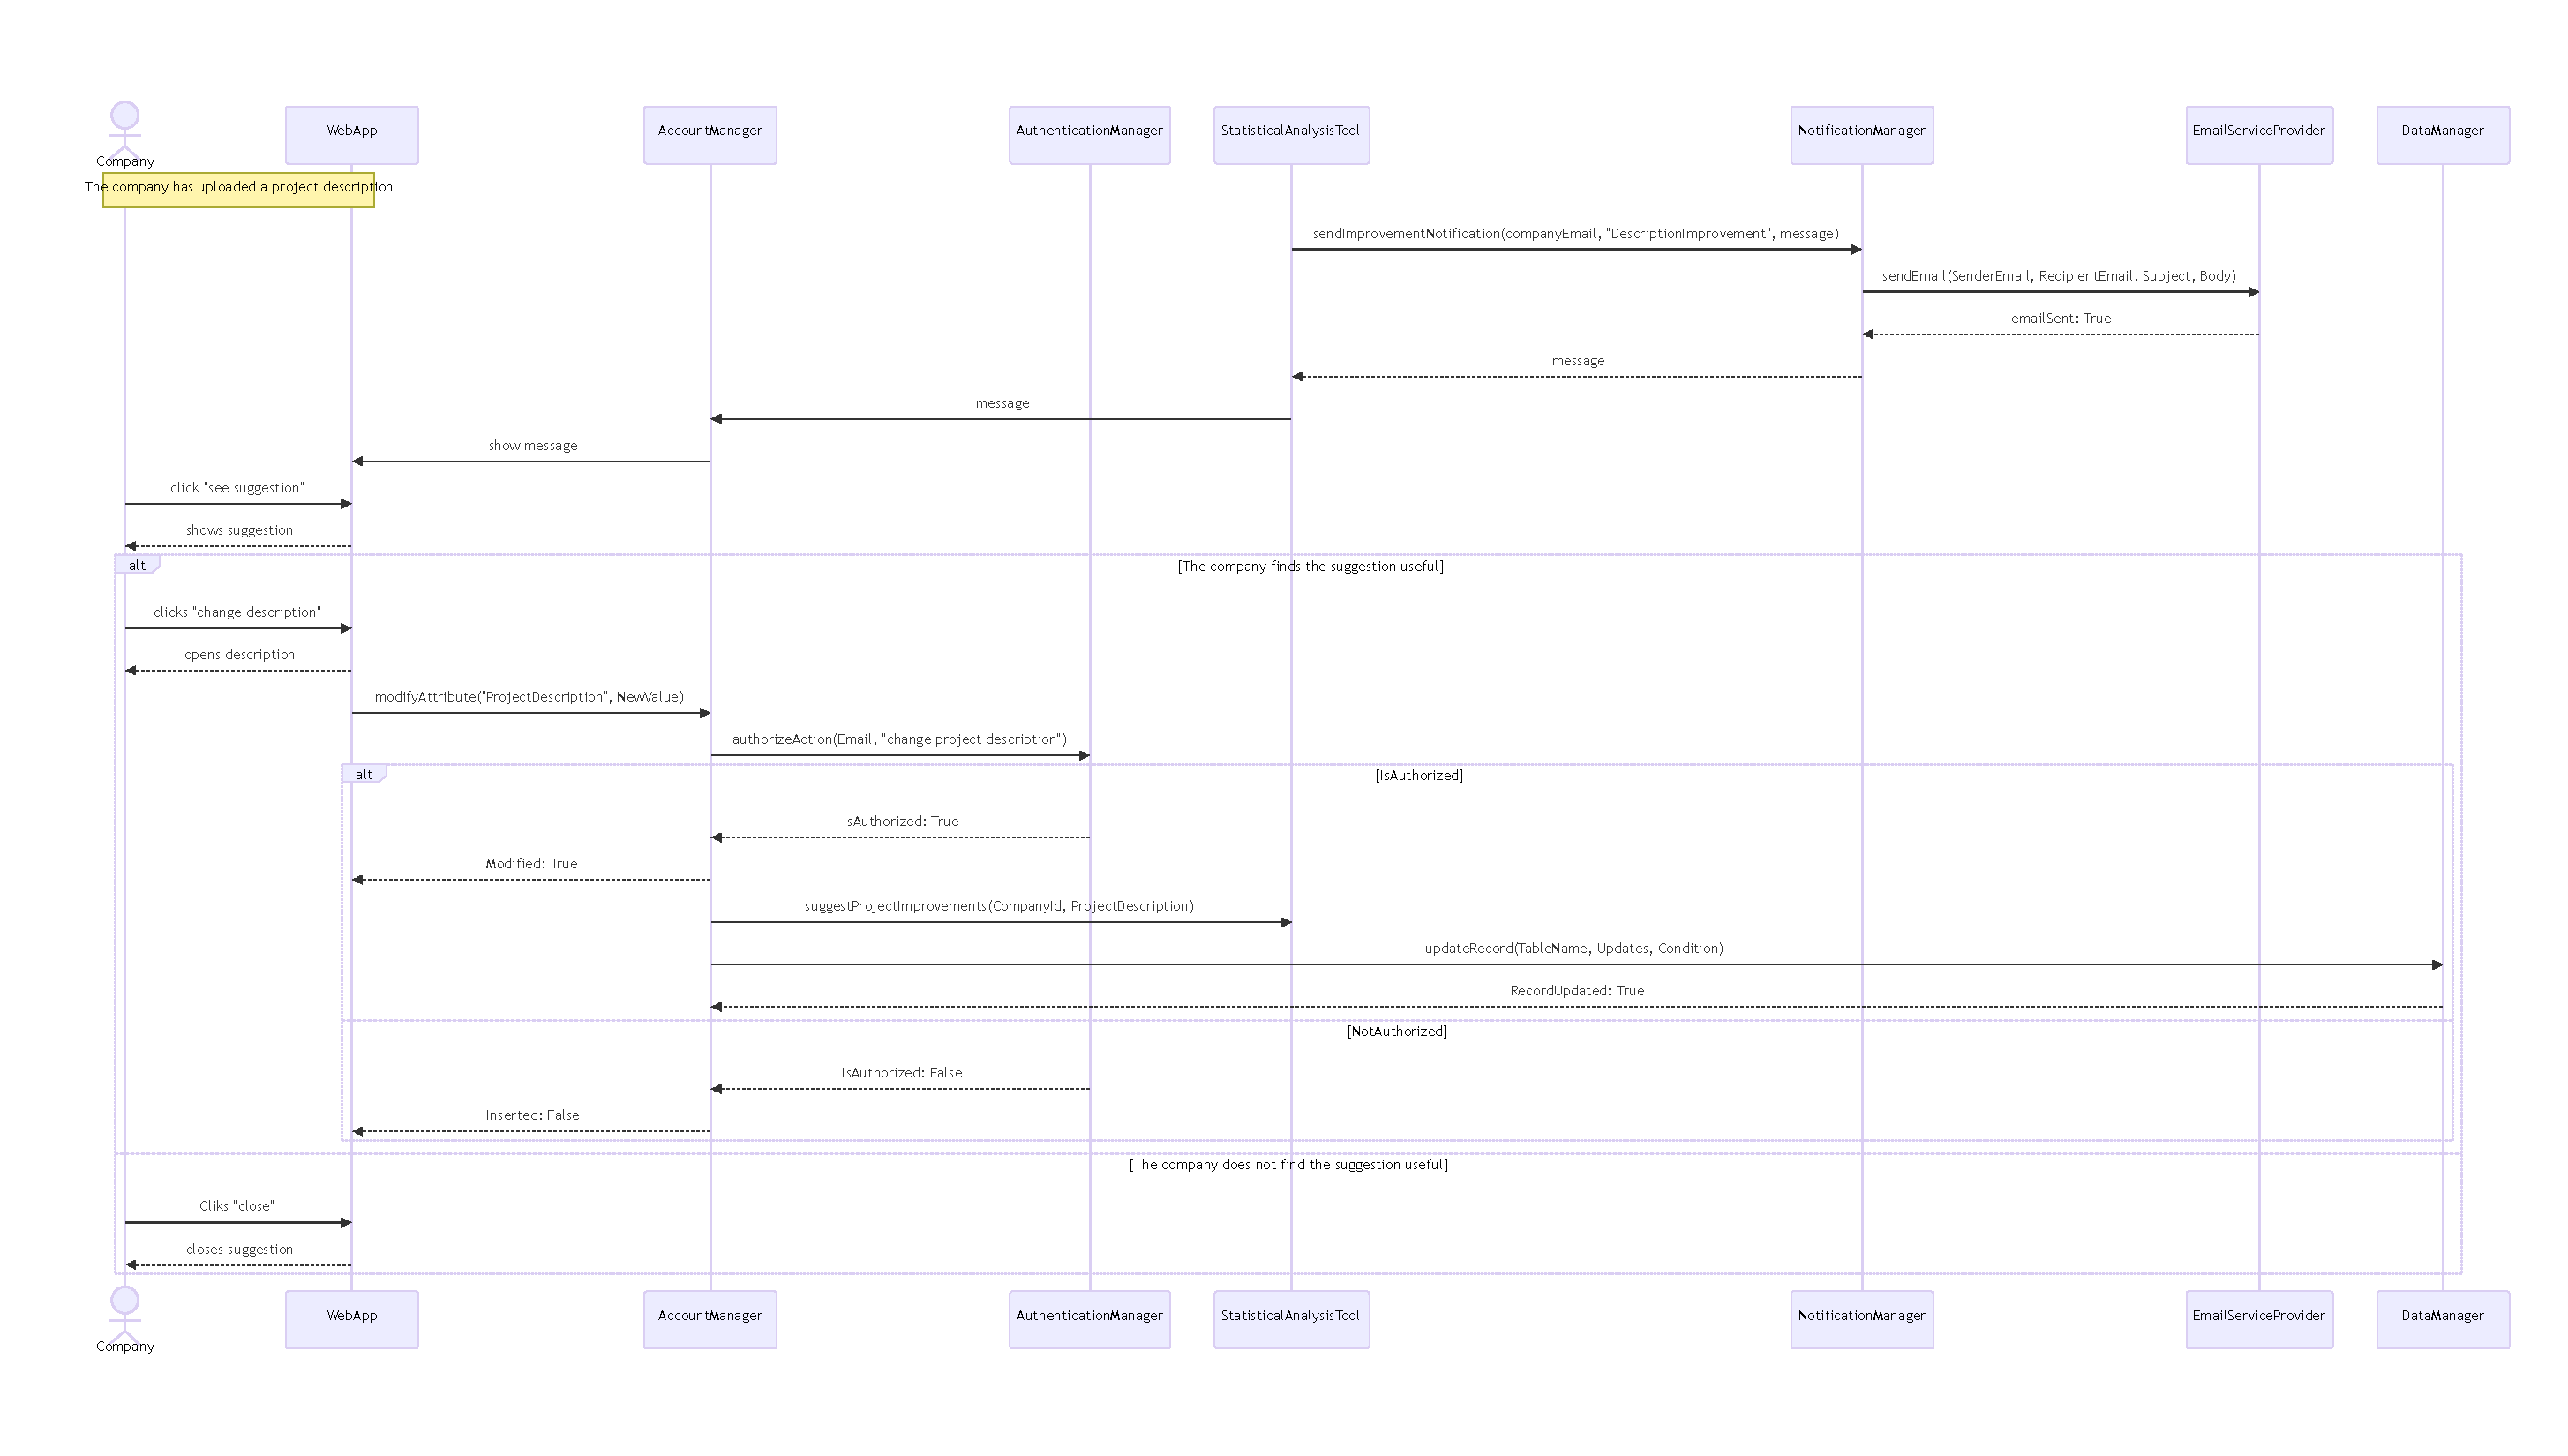
\includegraphics[width=1.1\linewidth]{DD//Images/SequenceDiagrams/UC9.pdf}
    \caption{UC9}
\end{figure}

\newpage
\textbf{UC10: User makes a complaint}

This sequence diagram describes the process in which a user interacts with the web app to monitor and leave complaints about their ongoing internship. The user navigates to the "Internships to Monitor" section, views internship details, and submits a comment or complaint. The complaint is saved and a notification is sent to the university.

Once the university logs in, they review the internship and complaints. If the complaint is deemed important, the university contacts the participant to manage the issue, resolves the complaint, and updates its status. If the complaint is critical, the university may terminate the internship, sending notifications to all relevant parties.

\begin{figure}[H]
    \centering
    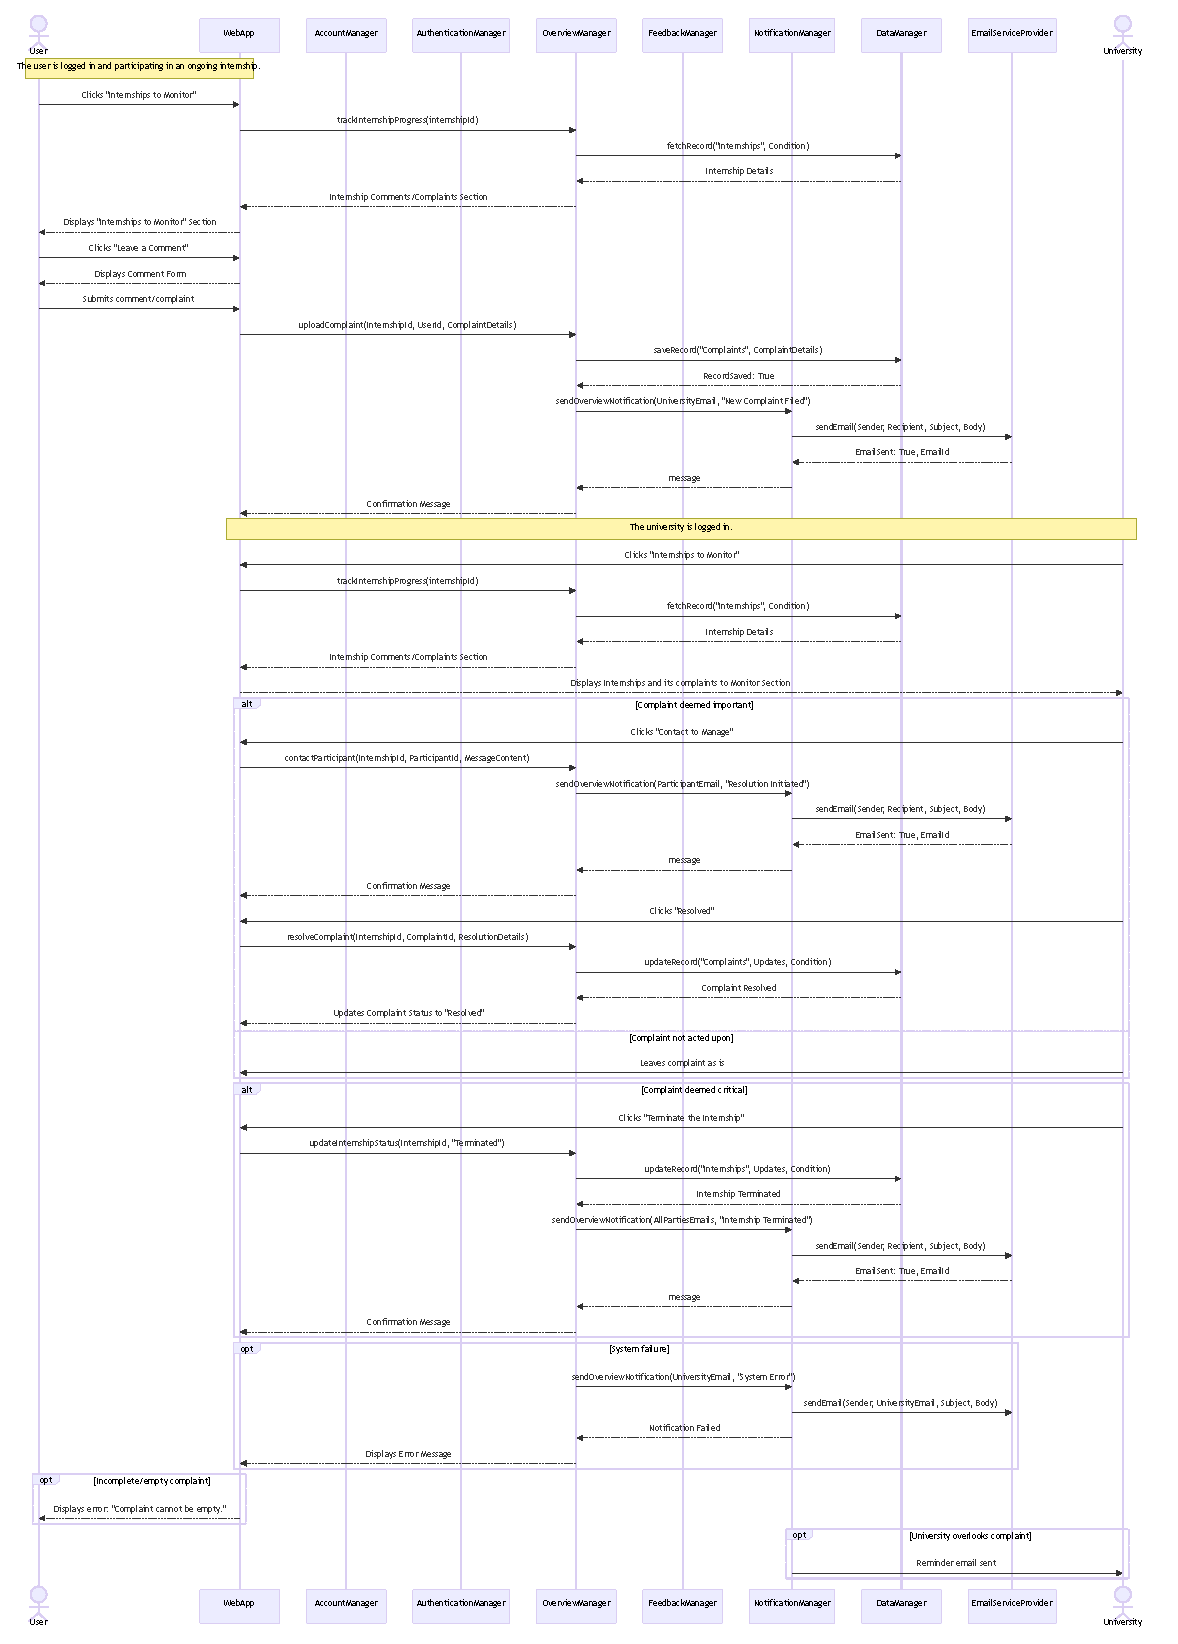
\includegraphics[width=0.9\linewidth]{DD//Images/SequenceDiagrams/UC10.pdf}
    \caption{UC10}
\end{figure}






\section{Component interfaces}
The Component Interfaces here described are the ones exposed in the components. Only the most relevant method parameters and methods
are shown.


\begin{itemize}
\item \textbf{Account Manager Interface}
    \begin{itemize}
    \item \textbf{registerUserAsStudent(string Email, string Name, data BirthDate, string LocationBirth, string Password) : boolean AccountCreated}

    This method takes all the data in input and contacts the DataManager to register a new StudentUser in the system.

    \item \textbf{registerUserAsCompany(string Email, string CompanyName, string LocationAddress, string Password) : boolean AccountCreated}
    
    This method takes all the data in input and contacts the DataManager to register a new CompanyUser in the system.

    \item \textbf{registerUserAsUniversity(string Email, string UniversityName, string LocationAddress, string Password) : boolean AccountCreated}
    
    This method takes all the data in input and contacts the DataManager to register a new UniversityUser in the system.

    \item \textbf{loginUser(string Email, string Password) : boolean LoginSuccessful}
    
    This method takes the user's email and password, checks weather they are registered and if they are it logs them into their account

    \item \textbf{insertCv(CV Cv): boolean Inserted}
    
    This method allows a StudentUser to upload their Cv on their profile. 

    \item \textbf{deleteCv(): boolean Deleated}
    
    This method allows a StudentUser to delete their Cv from their profile.
    
    \item \textbf{insertProjectDescription(string ProjectDescription): booleand Inserted}
    
    This method allows a CompanyUser to upload a new project description on their profile.

    \item \textbf{deleteProjectDescription(string ProjectName): booleand Deleted}
    
    This method allows a CompanyUser to delete a project description from their profile.

    \item \textbf{modifyAttribute(string AttributeName, string NewValue): boolean Modified}
    
    This method allows users to modify any data present on their profile.
    \end{itemize}

\item \textbf{Authentication Manager Interface:}
\begin{itemize}

\item \textbf{authorizeAction(string Email, string Action) : boolean IsAuthorized, string UserId}  

This method determines whether the specified user has the necessary permissions to perform the given action. It returns `true` if the action is allowed, otherwise `false`.


\end{itemize}

\item \textbf{Feedback Manager Interface}
    \begin{itemize}

    \item \textbf{submitFeedback(string UserId, string FeedbackContent): boolean Submitted}

    This method allows users to submit their feedback. The content is processed and forwarded to the Statistical Analysis Tool for further use.

    \item \textbf{getFeedbackHistory(string UserId): list FeedbackList}

    This method retrieves the history of feedback provided by a specific user for review or analysis purposes.
    \end{itemize}
\item \textbf{Application Manager Interface:}
\begin{itemize}
    \item \textbf{submitApplication(string UserId, string InternshipId): boolean Submitted}

    This method allows a student to submit an application for a specified internship. It processes the application and records it in the system.

    \item \textbf{acceptRecommendationStudent(string UserId, string RecommendationId): boolean Accepted}

    This method processes a student's acceptance of a recommendation provided by the system and creates an application for the corresponding internship.

    \item \textbf{acceptRecommendationCompany(string UserId, string RecommendationId): boolean Accepted}

    This method processes a company's acceptance of a recommendation provided by the system and creates an invitation for the Student for the corresponding internship.

    \item \textbf{acceptRecommendationCompanyWhenStudentAlreadyApplied(string UserId, string RecommendationId): boolean Accepted}

    This method processes a company's acceptance of a recommendation provided by the system when the student has already applied to that position.
    
    \item \textbf{rejectRecommendationCompanyWhenStudentAlreadyApplied(string UserId, string RecommendationId): boolean Rejected}

    This method processes a company's rejection of a recommendation provided by the system when the student has already applied to that position.
    
    \item \textbf{respondToInvitation(string UserId, string InvitationId): boolean Responded}

    This method allows a student to respond to an invitation from a company and generates an application if the invitation is accepted.
\end{itemize}

\item \textbf{Interview Manager Interface:}
\begin{itemize}
    \item \textbf{createAssessmentForum(string CompanyId, string UserId, string AssessmentDetails): boolean Created}

    This method allows a company to create a forum for conducting a prior assessment with a student. The forum includes assessment details and discussion tools for evaluations.

    \item \textbf{resolveAssessment(string ForumId, string ResolutionDetails): boolean Resolved}

    This method finalizes the outcome of a prior assessment conducted in the forum and records the resolution in the system.

    \item \textbf{evaluateAssessment(string ForumId, string EvaluationFeedback): boolean Evaluated}

    This method records feedback and evaluations on the assessment process, providing insights for both the student and the company.
    
    \item \textbf{scheduleInterview(string UserId, string CompanyId, datetime InterviewDate): boolean Scheduled}

    This method schedules an interview between a student and a company and records the details in the system.

    \item \textbf{updateInterviewStatus(string InterviewId, string Status): boolean Updated}

    This method allows updating the status of an interview (e.g., scheduled, completed, canceled) and ensures the system reflects the current progress.

    \item \textbf{finalizeSelection(string CompanyId, string UserId): boolean Finalized}

    This method records the final selection decision made by the company and updates the relevant data.

    
    \item \textbf{initiateContact(string StudentEmail, string CompanyEmail): boolean Contacted}

    This method is used by the community to initiate the first contact with the student; it calls the NotificationManager to do so.
    
\end{itemize}
\item \textbf{Recommendation Manager Interface:}
\begin{itemize}
    \item \textbf{newMatchFount(studentId, companyId): Boolean matchRecieved}

    This method is called by the StatisticalAnalysisTool when a new match is found and is used to notify both parties.

    \item \textbf{deleteMatch(studentId, companyId): Boolean matchDeleted}

    This method is called by the WebApp when a student or a company rejects a match, it then calls operations from other managers to delete the match from the system and notify the parties involved.
\end{itemize}
\item \textbf{Overview Manager Interface:}
\begin{itemize}
    \item \textbf{trackInternshipProgress(string InternshipId): map ProgressData}

    This method retrieves the current progress data for a specific internship, including details about the student, company, and related activities.

    \item \textbf{updateInternshipStatus(string InternshipId, string StatusUpdate): boolean Updated}

    This method updates the status of an ongoing internship (e.g., in progress, paused, completed) and records the changes in the system.

    \item \textbf{logInternshipUpdate(string InternshipId, string UpdateDetails): boolean Logged}

    This method registers detailed updates regarding the internship in the database. It communicates with the Authentication Manager for permission and the Data Manager to store the data.

    \item \textbf{uploadComplaint(string InternshipId, string UserId, string ComplaintDetails): boolean Uploaded}

    This method allows students or companies to file a complaint about the internship. The complaint is logged in the system for review and resolution by the university.

    \item \textbf{resolveComplaint(string InternshipId, string ComplaintId, string ResolutionDetails): boolean Resolved}

    This method allows universities to resolve complaints raised during the internship. Resolutions are documented and communicated back through the app.

    \item \textbf{reportComplaintOutcome(string InternshipId, string ComplaintId): boolean Reported}

    This method updates the system with the outcome of externally resolved complaints, ensuring all data remains centralized and accessible.

    \item \textbf{contactParticipant(string InternshipId, string ParticipantId, string MessageContent): boolean Contacted}

    This method enables the university to directly contact a student or company involved in the internship by sending a message through the app.

\end{itemize}

\item \textbf{StatisticalAnalysisTool Manager Interface:}
\begin{itemize}

    \item \textbf{generateStudentMatches(string StudentId): list Matches}

    This method generates a list of potential matches between students and internship projects based on student CVs and project descriptions using the recommendation system.

    \item \textbf{generateCompanyMatches(string ProjectId): list Matches}

    This method generates a list of potential matches between students and internship projects based on student CVs and project descriptions using the recommendation system.

    \item \textbf{suggestCvImprovements(string StudentId, CV Cv): list Suggestions}

    This method analyzes a student's CV and provides personalized suggestions for improvements to enhance their profile and compatibility with internship opportunities.

    \item \textbf{suggestProjectImprovements(string CompanyId, string ProjectDescription): list Suggestions}

    This method evaluates a company's project description and provides recommendations for making it more appealing and clear to potential candidates.

    \item \textbf{refineRecommendations(string FeedbackData): boolean Refined}

    This method processes feedback received from students and companies about previous recommendations to update and improve the recommendation algorithm.

    \item \textbf{fetchData(string DataRequest): map Data} 

    This method interacts with the Data Manager to retrieve necessary data for analysis, ensuring access permissions are obtained through the Authentication Server.

    \item \textbf{newApplication(string ApplicationData): boolean Recieved}

    This method is called when a new application is done by a student and the StatisticalAnalysisTool needs to know it. It then calls the data manager interface to update the database.

    \item \textbf{deleteMatch(string StudentId, string CompanyId): boolean Deleted}

    This method deletes a match that was found by this system if it was rejected by one or more parties.

    \item \textbf{newFeedback(string UserTd, string Feedback): boolean Recieved}

    This method is called by the FeedbackManager when there is new feedback given by a user to be analyzed. 
    \end{itemize}


\item \textbf{Notification Manager Interface:}
\begin{itemize}
    \item \textbf{sendAccountNotification(userEmail: String, notificationType: String, message: String): String message}

    This method is used to send notifications related to account activities, such as registration confirmations, password updates, or account deactivations. It’s typically called by the Account Manager.
    The method takes the userEmail (the ID of the user to notify), a notificationType (like "Registration"), and a message containing the notification content. The message is both sent by email through the notification manager and the Account Manager receives the formatted message through the backward chain and passes it along to the WebApp, where it’s displayed to the user in the notification page.
    \item \textbf{sendFeedbackNotification(userEmail: String, feedbackType: String, message: String): String message
}

    This method is used to send notifications requesting or acknowledging user feedback, such as a prompt to review an internship. It’s typically called by the Feedback Manager.
    The method takes the userEmail (the email of the user to notify), a feedbackType (like "InternshipFeedback"), and a message containing the notification content. The message is sent by email through the Notification Manager, and the Feedback Manager receives the formatted message through the backward chain and passes it along to the WebApp, where it is displayed to the user to encourage engagement.

    \item \textbf{sendImprovementNotification(userEmail: String, improvementType: String, message: String): String message
}

    This method is used to send notifications on improvements on a student's CV or a company's project description that the StatisticalAnalysisTool found.
    The method takes the userEmail (the email of the user to notify), a improvementType (like "CVFeedback"), and a message containing the notification content. The message is sent by email through the Notification Manager.
    \item \textbf{sendRecommendationNotification(userEmail: String, recommendationDetails: String): String message
}

    This method is used to send notifications about internship recommendations to students or companies, informing them about relevant matches. It’s typically called by the Recommendation Manager.
    The method takes the userEmail (the email of the user to notify) and recommendationDetails (like "You have been recommended for the Software Engineer position at TechCorp"). The message is sent by email through the Notification Manager, and the Recommendation Manager receives the formatted message through the backward chain and passes it along to the WebApp, where the user is notified about the recommendation on their dashboard.
    \item \textbf{sendApplicationNotification(userEmail: String, applicationStatus: String, message: String): String message}

    This method is used to notify users about updates related to their internship applications, such as submission confirmations, acceptance, or rejections. It’s typically called by the Application Manager.
    The method takes the userEmail (the email of the user to notify), an applicationStatus (like "Submitted" or "Accepted"), and a message detailing the update. The message is sent by email through the Notification Manager, and the Application Manager receives the formatted message through the backward chain and passes it along to the WebApp, where the user sees the application update on the notification page.
    \item \textbf{sendInterviewNotification(userEmail: String, interviewDetails: String): String message}

    This method is used to notify users about interview-related updates, such as scheduling, rescheduling, or cancellations. It’s typically called by the Interview Manager.
    The method takes the userEmail (the email of the user to notify) and interviewDetails (like "Your interview is scheduled for July 5th at 3:00 PM"). The message is sent by email through the Notification Manager, and the Interview Manager receives the formatted message through the backward chain and passes it along to the WebApp, where the user sees the interview details on their notification page.
    \item \textbf{sendOverviewNotification(userEmail: String, progressUpdate: String): String message}

    This method is used to notify users about updates on the progress of ongoing internships, ensuring students, universities, and companies are informed about important milestones. It’s typically called by the Overview Manager.
    The method takes the userEmail (the email of the user to notify) and a progressUpdate (like "Your student has reached 80\% of the internship goals"). The message is sent by email through the Notification Manager, and the Overview Manager receives the formatted message through the backward chain and passes it along to the WebApp, where it’s displayed on the notification page for relevant users.

    \item \textbf{sendGeneralNotification(userEmail: string, toUserIds: List[String], message: String): String message}
    
    This method is used for sending generic notifications that don’t fit into other specific categories. It supports notifications across various channels and can target multiple users simultaneously. It’s called by any module requiring an ad hoc notification.
    The message is sent by the Notification Manager, and the calling module receives the formatted message through the backward chain and passes it along to the WebApp, where it’s displayed in the user’s notification area.


\end{itemize}


\item \textbf{Data Manager:}
\begin{itemize}

\item \textbf{checkDuplicates(string TableName, string Email) : boolean Duplicates}

This method when called checks if the email inserted already exists in the database.
    
\item \textbf{saveRecord(string TableName, map<string, string> Data) : boolean RecordSaved}  

This method saves a new record in the specified table. It returns `true` if the record is successfully stored.

\item \textbf{fetchRecord(string TableName, string Condition) : map<string, string> FetchedRecord}  

This method retrieves a single record from the specified table that matches the provided condition. Returns the record as a key-value map.

\item \textbf{fetchAllRecords(string TableName, string Condition) : list<map<string, string>> RecordsList} 

This method retrieves all records from the specified table that match the provided condition. Returns the data as a list of key-value maps.

\item \textbf{updateRecord(string TableName, map<string, string> Updates, string Condition) : boolean RecordUpdated}  

This method updates records in the specified table based on the condition provided. Returns `true` if the update is successful.

\item \textbf{deleteRecord(string TableName, string Condition) : boolean RecordDeleted}  

This method deletes records from the specified table that match the provided condition. Returns `true` if the deletion is successful.

\item \textbf{provideDataAccess(string ModuleName, string DataRequest) : map<string, string> AccessedData}  
This method grants secure data access to a specific module, returning the requested data while enforcing access control policies.

\end{itemize}

\item \textbf{Email Service Provider: }
\begin{itemize}
\item \textbf{sendEmail(string SenderEmail, string RecipientEmail, string Subject, string Body) : boolean EmailSent, string EmailId} 

This method sends an email to the specified recipient with the provided subject and body content. Returns `true` if the email is successfully sent.

\item \textbf{sendTemplatedEmail(string SenderEmail, string RecipientEmail, string TemplateName, map<string, string> TemplateData) : boolean EmailSent, string EmailId}  

This method sends an email using a predefined template. It takes the template name and a mapping of dynamic data to populate the template fields.

\item \textbf{trackEmailDelivery(string EmailId) : string DeliveryStatus} 

This method checks the delivery status of a previously sent email using its unique email ID. It returns statuses such as "Delivered," "Failed," or "Pending."

\item \textbf{configureEmailSettings(string SMTPServer, int Port, string SenderEmail, string SenderPassword) : boolean SettingsConfigured}  

This method configures the SMTP settings for sending emails, including the server address, port, sender email, and authentication details.

\item \textbf{validateEmailAddress(string EmailAddress) : boolean IsValid}  

This method checks whether the given email address is in a valid format and can be used for sending emails.

\item \textbf{resendFailedEmails(string[] FailedEmailIds) : boolean Resent}  

This method retries sending emails that previously failed to be delivered. Returns `true` if all retries are successful.
\end{itemize}

\item \textbf{DBMS:}
\begin{itemize}
\item \textbf{postData(string TableName, map<string, string> Data) : boolean IsStored} 

This method inserts the provided data into the specified table within the database. Returns `true` if the operation is successful.

\item \textbf{getData(string Query) : list<map<string, string > > RetrievedData}  

This method executes the provided query to fetch data from the database. It returns the results as a list of records.

\item \textbf{updateData(string TableName, map<string, string> Updates, string Condition) : boolean IsUpdated}

This method updates records in the specified table based on the condition provided. Returns `true` if the update is successful.

\item \textbf{deleteData(string TableName, string Condition) : boolean IsDeleted}  

This method removes records from the specified table that match the provided condition. Returns `true` if the deletion is successful.

\item \textbf{manageAccessControl(string UserId, string[] Permissions) : boolean AccessManaged}  

This method updates access control policies for a specific user by assigning or revoking permissions.

\end{itemize}
\end{itemize}


\pagebreak
\section{Selected architectural styles and patterns}

\subsection{Three Tier Architecture}
In the Students \& Companies project, we chose a three-tier architecture as explained in Section 2.1. This architecture separates the system into three layers (or tiers) : the Presentation layer, the Application layer, and the Data layer. For this implementation, we opted for a remote presentation layer, where the graphical user interface (GUI) resides entirely on the client side, such as in a web browser or a mobile app. This decision brings several advantages: it reduces the server's workload by allowing it to focus on processing business logic and managing data, improves the responsiveness of the user interface since it is processed locally on the user’s device, and reduces bandwidth usage while improving network efficiency.

The three-tier architecture distributes responsibilities effectively within the Students \& Companies application. The Presentation tier handles all user interactions, providing a seamless interface for students, companies, and universities to input and access data. The Application tier serves as the processing hub, managing tasks like user authentication, recommendation algorithms, and communication between the user interface and the database. Finally, the Data tier is responsible for securely storing and managing essential data, such as user profiles, CVs, project descriptions, and application histories, while performing all database operations to ensure reliability and data integrity.

The primary benefit of using a three-tier architecture, and the reason it was chosen for the Students \& Companies system, is its modularity. Each tier can be developed, maintained, and operated independently on separate infrastructures. This separation simplifies updates and extensions by allowing modifications to be made to one tier without affecting the others. It enhances scalability and performance, making it easier to handle increased loads, and provides flexibility for evolving and adapting the system to future needs while maintaining its reliability and stability.

\pagebreak
\subsection{Component Based Development}
Our approach is component-based, meaning the system is built using distinct, independent components that each handle specific functionalities. This approach offers significant advantages both in the short and long term. For example, by defining and developing components like the Application Manager or Feedback Manager, each responsible for a specific task, we can work on them independently without affecting the rest of the system. This modularity makes it easier to maintain, update, or even replace individual components without disrupting the entire system.  

\subsection{REST Architecture}
Our architecture is designed around REST principles, ensuring a stateless system where the server processes each request independently, while the client manages its own state. This approach improves scalability and efficiency by decoupling state management from the server, enabling each request to include all the necessary information for processing. A significant advantage of this design is cacheability: frequently accessed data, such as internship listings or static resources, can be cached, reducing server load and improving response times for users.

The REST architecture also ensures a uniform interface, with APIs designed around resources rather than actions. Endpoints like /emails, /data, or /records allow operations through standard HTTP methods (GET, POST, PUT, DELETE), providing a consistent and predictable structure across the system. The methods we declared in the APIs, such as sendEmail and postData, are our custom implementations and are mapped to RESTful operations (e.g., POST for creating resources or GET for retrieving them), ensuring that the system aligns with REST principles while retaining flexibility.

Additionally, REST aligns perfectly with our modular and scalable deployment architecture. The stateless nature of REST makes it easy to distribute requests across multiple servers using a load balancer, ensuring efficient handling of high traffic. By adopting a hybrid approach, combining preconfigured services (e.g., for email handling) with custom RESTful endpoints, the system achieves flexibility while adhering to REST principles. Overall, REST provides the scalability, adaptability, and consistency required to meet the needs of the Students \& Companies platform and its users.

\subsection{Model View Controller}
The Model-View-Controller (MVC) pattern is a great fit for our system and works well with the architecture choices we've made. It divides the application into three distinct layers: the Model manages the data (consistent with the Data Layer in our three-tier architecture), the View handles user interaction and display (aligned with the Presentation Layer), and the Controller connects both the data and the user interface (matching the Application Layer’s role of processing business logic).

By using MVC, we maintain the modularity and separation of concerns we discussed earlier with the three-tier architecture. The MVC pattern enhances our ability to scale and maintain the system since each layer can evolve independently. For instance, we can modify the user interface (View) or improve the application logic (Controller) without impacting how the data is managed (Model). Additionally, MVC supports the RESTful principles we implemented, ensuring that each request is stateless and can be handled independently. This consistency between architectural choices ensures that the application remains flexible, maintainable, and easily adaptable to future changes.

\pagebreak
\section{Other design decisions }
\subsection{MongoDB}

We chose to implement our databases using a NoSQL model, specifically MongoDB, as it is well-suited for modern web applications that require scalability, flexibility, and fast development cycles. MongoDB’s schema-less design allows us to handle evolving data requirements effectively and simplifies integration with our architecture.

 we divided the data into three distinct collections within separate MongoDB databases:

\begin{itemize}
    \item \textbf{User Database:} This database is responsible for managing user-related data, including profiles for both students and companies, login credentials, and session details. It is accessed during user authentication (login/registration) and session management. MongoDB’s document model allows us to store and query diverse user types efficiently while adapting to changing data requirements.
    \item \textbf{Opportunities Database:} This database handles all data related to internship opportunities, including job postings, candidate recommendations, invitations, and match notifications. Each request involving the creation, update, or retrieval of internship-related data interacts with this database. MongoDB’s flexible schema is ideal for storing hierarchical data, such as job descriptions, candidate lists, and interview schedules, in a single, cohesive structure.
    \item \textbf{Internship Feedback Database:} This database manages feedback and issue tracking during internships. It stores data related to feedback from students, companies, and universities, as well as complaint logs and resolution updates. The use of embedded documents ensures that related feedback and complaint data can be stored together for efficient access and analysis
\end{itemize}

MongoDB was chosen for its scalability, built-in sharding for distributing data across servers, and support for advanced aggregation pipelines, which are ideal for handling complex queries efficiently. 
\chapter{User Interface Design}


This section presents screenshots of the Students and Companies app, highlighting its interface and key features, giving a clear view of how users interact with the platform.

\begin{figure}[H]
    \centering
    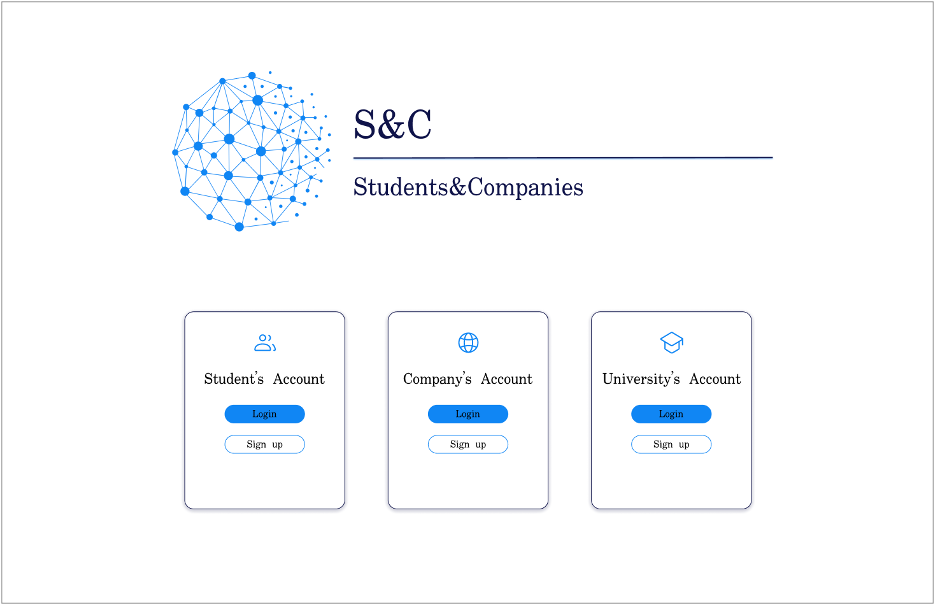
\includegraphics[width=1\linewidth]{DD//Images/UI photos/Home.png}
    \caption{Login Page}
\end{figure}

The Login Page allows users to choose whether to create a new account or log into an existing one. Users can select their role (student, company, or university) to access the appropriate features of the app.

\begin{figure}[H]
    \centering
    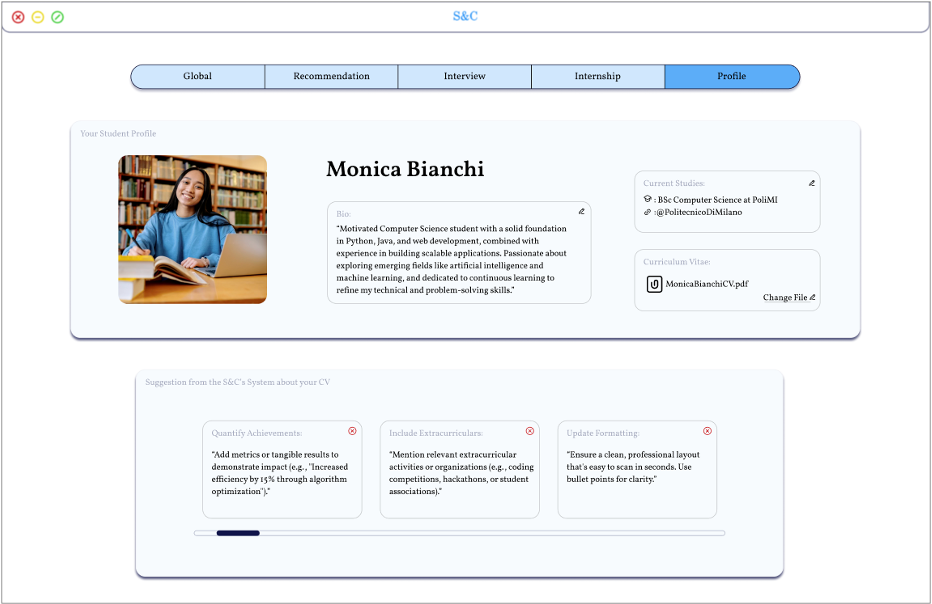
\includegraphics[width=1\linewidth]{DD//Images/UI photos/Student's Profile.png}
    \caption{Student's Profile Page}
\end{figure}

The Student's Profile Page displays the student's photo, bio, and education information, with options to view and update this information. It also allows the student to upload, delete, or re-upload their CV. Below the profile details, the page shows personalized suggestions from the Students and Companies system, offering hints to improve their CV.


\begin{figure}[H]
    \centering
    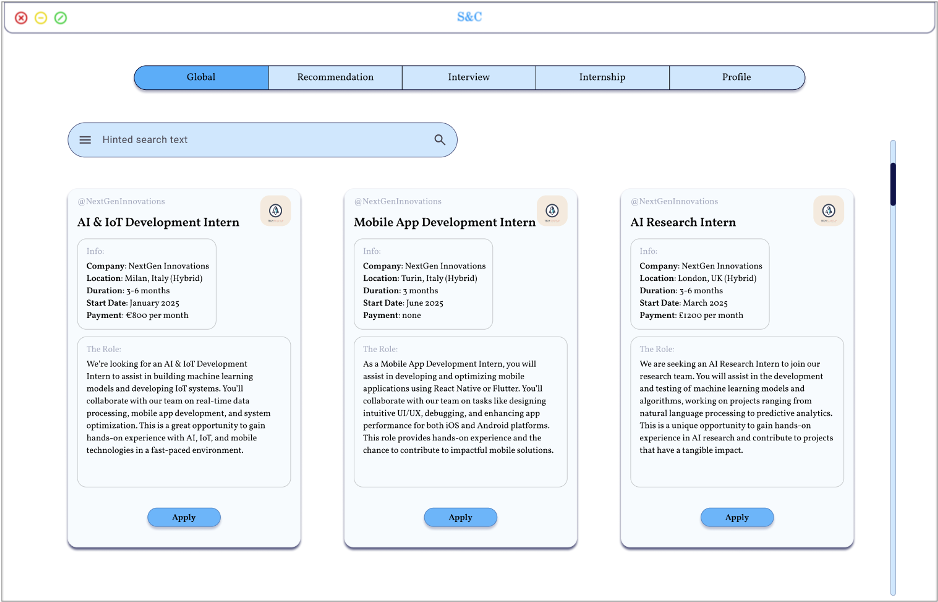
\includegraphics[width=1\linewidth]{DD//Images/UI photos/Student's Global.png}
    \caption{Student's Global Searching Page}
\end{figure}

The Student's Global Searching Page allows students to browse all available internship project descriptions. They can proactively search for internships that match their interests and skills, using keywords or specific parameters. Students also have the option to apply directly to internships that suit them best.

\begin{figure}[H]
    \centering
    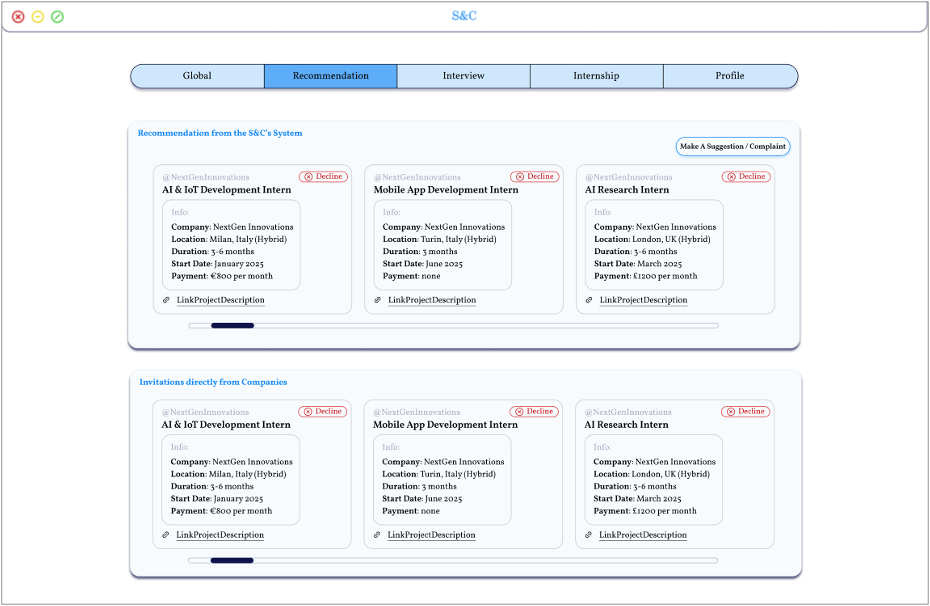
\includegraphics[width=1\linewidth]{DD//Images/UI photos/Student's Recommendations.png}
    \caption{Student's Recommendations Page}
\end{figure}

The Student's Recommendations Page displays internship opportunities suggested by the Students and Companies system, tailored to the student's profile. The student can accepts the recommendation applying for the position. Below these recommendations, the student can also view invitations sent directly from companies. In both cases, the student can apply directly to the internships.

\begin{figure}[H]
    \centering
    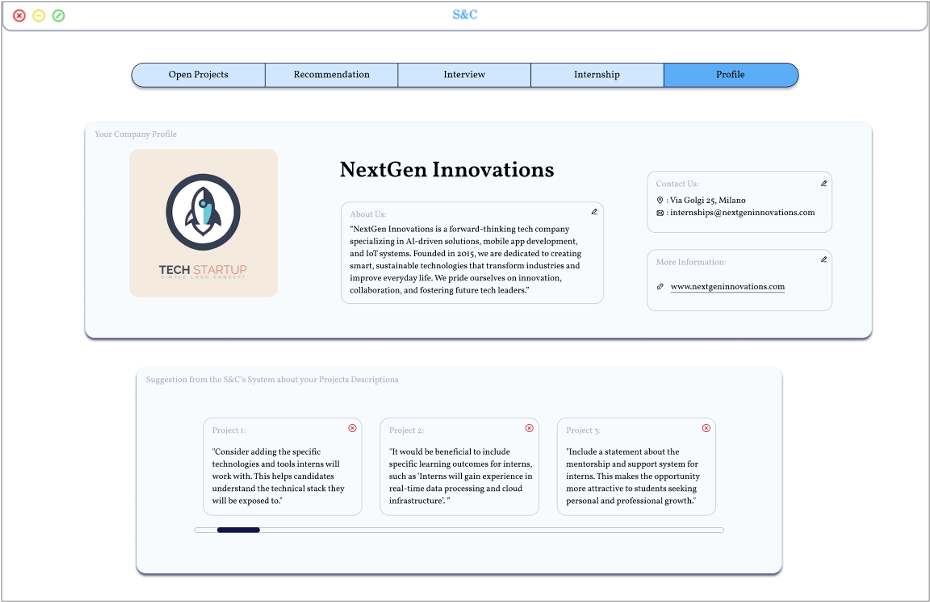
\includegraphics[width=1\linewidth]{DD//Images/UI photos/Company's Profile.png}
    \caption{Company's Profile Page}
\end{figure}

The Company's Profile Page displays the company's bio and all the information they’ve provided about themselves, with the option to edit and update this content. Below, the page shows suggestions from the Students and Companies system on how to improve the descriptions of each posted internship project, making them more appealing and informative.

\begin{figure}[H]
    \centering
    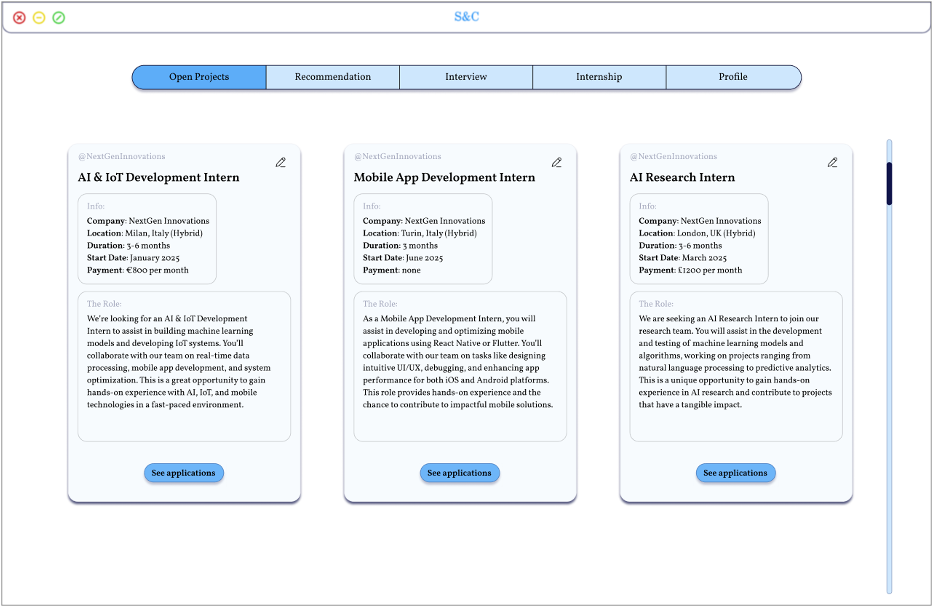
\includegraphics[width=1\linewidth]{DD//Images/UI photos/Company's Projects.png}
    \caption{Company's open projects Page}
\end{figure}

The Company's Open Projects Page displays all the internship project descriptions that the company has published. It offers the option to modify these descriptions and provides direct links to view the applications received for each internship.

\begin{figure}[H]
    \centering
    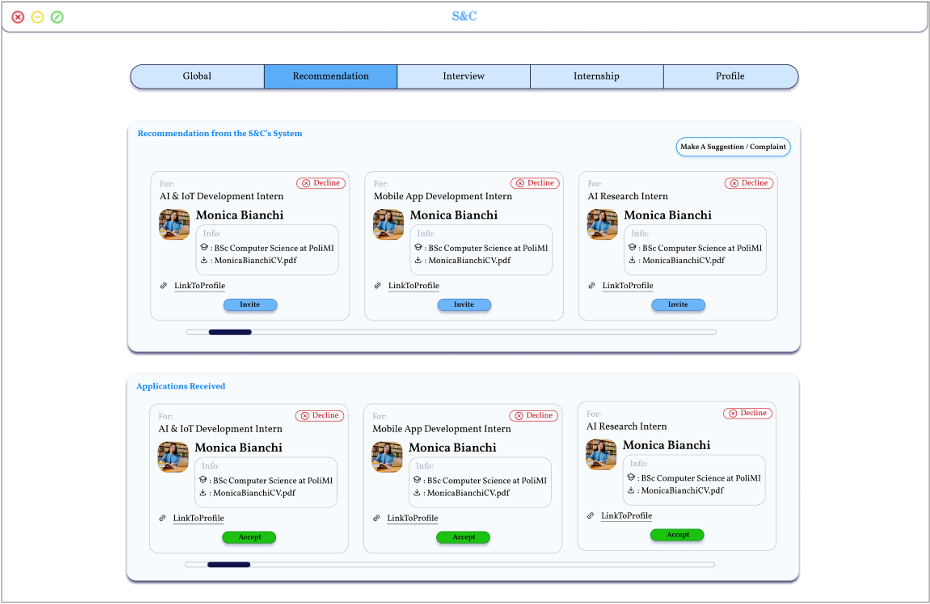
\includegraphics[width=1\linewidth]{DD//Images/UI photos/Company's reccomendations.png}
    \caption{Company's Recommendations Page}
\end{figure}

The Company's Recommendations Page displays a list of recommended candidates from the system, providing a preview of their profiles with a direct link to view more details. The company can accept recommendations and invite students to apply. Below the recommendations, the page also shows all the applications the company has received from students.

\begin{figure}[H]
    \centering
    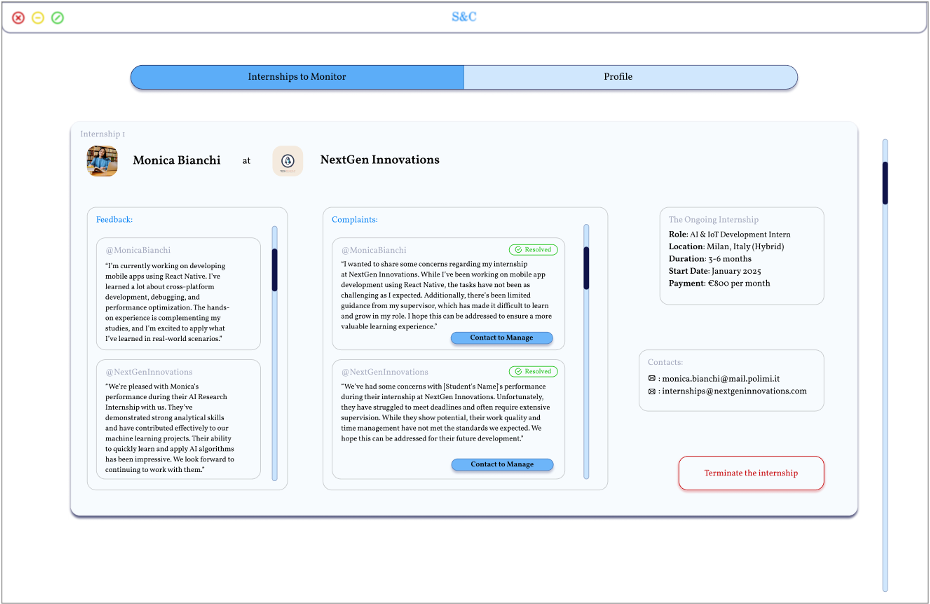
\includegraphics[width=1\linewidth]{DD//Images/UI photos/Universities Monitoring.png}
    \caption{University's ongoing internship Monitoring Page}
\end{figure}

The University's Ongoing Internship Monitoring Page provides a comprehensive overview of all ongoing internships, including details about the student, company, role, and relevant contact information. The page features sections for both feedback and complaints, which can be submitted by either the student or the company. Complaints can be managed within the app or resolved externally, with the option to report the resolution back on the platform.
\chapter{Requirements Traceability}
This chapter outlines the traceability framework implemented to maintain alignment between the project objectives, stakeholder needs, and the final deliverables. Establishing clear links between requirements, design, implementation, and testing minimizes the risk of unfulfilled specifications and promotes a transparent development process.

\textbf{[R1]} The system allows unregistered users to create an account.  
\begin{itemize}
    \item \textbf{WebApp:} Provides the user interface for new users to enter their registration details.
    \item \textbf{AccountManager:} Manages the account creation process, validates user details, and ensures proper storage of data.
    \item \textbf{AuthenticationManager:} Verifies that the registration process complies with security protocols.
    \item \textbf{DataManager:} Handles the storage of new user data in the database.
    \item \textbf{NotificationManager:} Sends notifications to users about the successful creation of their accounts.
    \item \textbf{EmailServiceProvider:} Sends email confirmation or verification messages to new users.
    \item \textbf{DBMS:} Stores all account information securely in the database.
\end{itemize}

\textbf{[R2]} The system allows students to upload their CV.  
\begin{itemize}
    \item \textbf{WebApp:} Provides the interface for students to upload their CVs.
    \item \textbf{AccountManager:} Ensures that only authenticated students can upload their CVs.
    \item \textbf{AuthenticationManager:} Validates the session and permissions of the student uploading the CV.
    \item \textbf{DataManager:} Stores the uploaded CV securely in the database.
    \item \textbf{StatisticalAnalysisToolManager:} Analyzes the CV to improve recommendations and provide insights for better matching.
    \item \textbf{DBMS:} Stores CV data for future reference and analysis.
\end{itemize}

\textbf{[R3]} The system allows companies to publish new internships.  
\begin{itemize}
    \item \textbf{WebApp:} Provides the interface for companies to add new internship postings.
    \item \textbf{AccountManager:} Ensures only authenticated company representatives can post internships.
    \item \textbf{AuthenticationManager:} Verifies that the company representative has the necessary permissions.
    \item \textbf{DataManager:} Stores the internship postings in the database.
    \item \textbf{StatisticalAnalysisToolManager:} Analyzes the internship postings to improve matching with student profiles.
    \item \textbf{DBMS:} Safely stores internship data for future searches and recommendations.
\end{itemize}

\textbf{[R4]} The system allows companies to add a description to their internships.  
\begin{itemize}
    \item \textbf{WebApp:} Provides the interface for adding detailed descriptions to internships.
    \item \textbf{AccountManager:} Verifies that authenticated companies can update internship details.
    \item \textbf{AuthenticationManager:} Checks permissions for modifying internship descriptions.
    \item \textbf{DataManager:} Updates and stores the descriptions in the database.
    \item \textbf{StatisticalAnalysisToolManager:} Uses the descriptions to refine internship recommendations for students.
    \item \textbf{DBMS:} Safely records the updated internship details.
\end{itemize}

\textbf{[R5]} When students want to do proactive research, the system allows them to go through the available internships.  
\begin{itemize}
    \item \textbf{WebApp:} Displays a list of internships for students to browse through.
    \item \textbf{ApplicationManager:} Manages the search and retrieval of available internships.
\end{itemize}

\textbf{[R6]} When doing a search, the system allows users to filter internships.  
\begin{itemize}
    \item \textbf{WebApp:} Provides filtering options for criteria such as location, domain, and duration.
    \item \textbf{ApplicationManager:} Processes search queries and applies filters to display relevant results.
\end{itemize}

\textbf{[R7]} When finding an internship that suits their interests, the system allows students to apply for it.  
\begin{itemize}
    \item \textbf{WebApp:} Enables students to submit their applications through the platform.
    \item \textbf{ApplicationManager:} Manages the submission of applications and notifies the relevant company.
    \item \textbf{StatisticalAnalysisToolManager:} Tracks application data to refine matching and recommendations.
    \item \textbf{AuthenticationManager:} Verifies the permissions and authenticity of the student applying.
    \item \textbf{NotificationManager:} Notifies both the student and the company about the application status.
    \item \textbf{EmailServiceProvider:} Sends confirmation emails to both parties regarding the application.
\end{itemize}

\textbf{[R8]} When finding a CV that suits their interests, the system allows companies to request that student's application.  
\begin{itemize}
    \item \textbf{WebApp:} Allows companies to request applications from students through the interface.
    \item \textbf{ApplicationManager:} Processes company requests and sends notifications to the respective students.
    \item \textbf{StatisticalAnalysisToolManager:} Updates its data based on the company’s preferences and feedback.
    \item \textbf{AuthenticationManager:} Verifies the company's permissions before granting access to student data.
    \item \textbf{NotificationManager:} Notifies students about application requests from companies.
    \item \textbf{EmailServiceProvider:} Sends email notifications to students regarding company interest.
\end{itemize}

\textbf{[R9]} When a new internship that might interest some students becomes available, the system notifies them.  
\begin{itemize}
    \item \textbf{WebApp:} Displays notification messages to students about new internships.
    \item \textbf{RecommendationManager:} Identifies students who may be interested in the new internships.
    \item \textbf{StatisticalAnalysisToolManager:} Analyzes new internships and matches them with student profiles.
    \item \textbf{NotificationManager:} Sends real-time notifications about new opportunities.
    \item \textbf{EmailServiceProvider:} Sends email alerts to students about new internships.
\end{itemize}



\textbf{[R10]} When a student's CV that corresponds to a company's needs becomes available the system informs them. 
\begin{itemize}
     \item \textbf{Statistical analysis tool manager}: Used to find possible match between a student's CV and internships descriptions posted by the Company.
     \item \textbf{Data Manager}: Used to access to both the student's CV and the company's internship's project description.
    \item \textbf{Recommendation Manager}: Compares the student's CV to the company's needs and identifies matches.
    \item \textbf{Notification Manager}: Sends notifications to the company once a matching CV is found.
    \item \textbf{Account Manager}: Lets the company visualize the before told CV.
    \item \textbf{Authentication Manager}: Ensures that the company is logged in a company type of account and has the privileges to do this action. 
\end{itemize}
\textbf{[R11]} The system allows students to accept a recommendation, applying for that particular internship. 
\begin{itemize}
    \item \textbf{Recommendation Manager}: Used to start the process protocol of when a student accepts a recommendation.
    \item \textbf{Data Manager}: Used to retrieve all the recommendation that were generated and linked to the student's profile.
    \item \textbf{Application Manager}: Takes care of sending and managing the student's application after he accepted the recommendation. 
    \item \textbf{Account Manager}: Shows possible recommendation and includes the student's details to the process of application.
    \item \textbf{Authentication Manager}: Ensures that the user is logged in a student type of account and has the privileges to do this action. 
    \item \textbf{Statistical analysis tool manager}: Register the acceptance feedback of the match it created to improve its effectiveness.
\end{itemize}
\textbf{[R12]} The system allows companies to accept a recommendation, inviting the candidate that was proposed.
\begin{itemize}
    \item \textbf{Recommendation Manager}: Manages the recommendation process and sends the company the proposed candidate's details
    \item \textbf{Account Manager}: tracks and shows to the company hich recommendations have been reviewed.
     \item \textbf{Data Manager}: Used to retrieve all the recommendation that were generated and linked to the company's profile.
    \item \textbf{Notification Manager}: Sends notifications to the proposed candidate once the company accepts the recommendation and extends the invitation.
    \item \textbf{Authentication Manager}: Ensures that the company is logged in a company type of account and has the privileges to do this action. 
    \item \textbf{Statistical analysis tool manager}: Register the acceptance feedback of the match it created to improve its effectiveness.
    
\end{itemize}
\textbf{[R13]} The system allows students to accept an invitation of a company for a particular internship, applying for it.
\begin{itemize}
    \item \textbf{Account Manager}: Handles the student’s action of accepting the invitation from a company and ensures their profile is up-to-date for the application while also linking the CV. 
    \item \textbf{Application Manager}: Facilitates the student’s submission of the internship application after accepting the invitation.
    \item \textbf{Notification Manager}: Sends notifications to the student to confirm the invitation and remind them to apply.
     \item \textbf{Data Manager}: Used to retrieve all the invitation that were linked to the student's profile.
    \item \textbf{Authentication Manager}: Ensures that the user is logged in a student type of account and has the privileges to do this action. 
    \item \textbf{Statistical analysis tool manager}: Register the acceptance feedback of the match it created to improve its effectiveness.
    
\end{itemize}
\textbf{[R14]}  When the two parties have accepted a recommendation, when the company has accepted an application received, or when the student has accepted a company's invitation the system allows them to establish a contact
\begin{itemize}
    \item \textbf{Account Manager}: Manages the contact information for both the student and the company, ensuring both parties are ready to engage.
    \item \textbf{Statistical analysis tool manager}: Register the acceptance feedback of the match it created to improve its effectiveness.
    \item \textbf{Notification Manager}: Notifies both the student and the company that they can now establish contact after acceptance.
    \item \textbf{Interview Manager}: Assists in scheduling and managing communications related to interviews or further discussions.
    \item \textbf{Authentication Manager}: Ensures that both the company and the student have the privileges to do this action, based on their previous interactions.
    
\end{itemize}
\textbf{[R15]} When conducting an interview, the system supports the companies with the interview process
\begin{itemize}
    \item \textbf{Interview Manager}: Manages the interview process, including scheduling and tracking progress.
    \item \textbf{Notification Manager}: Sends interview reminders and updates to both students and companies.
    \item \textbf{Statistical analysis tool manager}: Follows related feedback to improve its effectiveness. 
    \item \textbf{Authentication Manager}: Ensures that both the company and the student have the privileges to do this action, based on their previous interactions.
\end{itemize}
\textbf{[R16]} When conducting an interview, the system supports the companies with the finalization of the selection
\begin{itemize}
    \item \textbf{Interview Manager}: Helps the company track the progress of interviews and finalize their decision.
    \item \textbf{Notification Manager}: Used to inform the student of the outcome of the interviewing process.
\end{itemize}
\textbf{[R17]} The system allows students and companies to provide feedback and suggestions to perform statistical analysis.
\begin{itemize}
    \item \textbf{Feedback Manager}: Collects and manages feedback from both students and companies.
    \item \textbf{Statistical Analysis Tool Manager}: Analyzes the feedback data and generates statistical reports for insights.
    \item \textbf{Notification Manager}: Used to request feedback form users.
    \item \textbf{Account Manager}: Retrieves and stores feedback linked to the appropriate student and company profiles.
    \item \textbf{Authentication Manager}: Ensures that both the company and the student have the privileges to do this action.
    
\end{itemize}
\textbf{[R18] }The system provides suggestions to students regarding how to make their CVs more appealing
\begin{itemize}
    \item \textbf{Statistical Analysis Tool Manager}: Analyzes student CVs and generates suggestions for improvement based on trends and the needs of companies.
    \item \textbf{Account Manager}: Retrieves and updates the student’s CV for analysis.
     \item \textbf{Data Manager}: Used to access to all the students corresponding CVs and all the companies project description published to make the analysis. 
    \item \textbf{Notification Manager}: Sends the student notifications with suggestions on how to improve their CV.

\end{itemize}
\textbf{[R19]} The system provides suggestions to companies regarding how to make their project descriptions more appealing
\begin{itemize}
    \item \textbf{Statistical Analysis Tool Manager}: Analyzes student CVs and generates suggestions for improvement based on trends and the needs of companies.
    \item \textbf{Account Manager}: Retrieves and updates the company's project description for analysis.
     \item \textbf{Data Manager}: Used to access to all the students corresponding CVs and all the companies' project description published to make the analysis. 
    \item \textbf{Notification Manager}: Sends the student notifications with suggestions on how to improve their CV.
\end{itemize}

\textbf{[R20]} During the matchmaking process, the system allows all users to keep track of its execution and outcome.
\begin{itemize}
    \item \textbf{Recommendation Manager}: Monitors the matchmaking process and tracks the outcomes for each user.
    \item \textbf{Statistical Analysis Tool Manager}: Provides detailed insights and progress tracking of matches during execution.
    \item \textbf{Notification Manager}: Updates users in real time about the status of the matchmaking process.
    \item \textbf{Account Manager}: Allows users to view ongoing matchmaking results in their accounts.
    \item \textbf{Authentication Manager}: Ensures access rights are respected when viewing matchmaking data.
\end{itemize}

\textbf{[R21]} During the internship, the system allows all interested parties to monitor it.
\begin{itemize}
    \item \textbf{Overview Manager}: Tracks the progress and updates of the ongoing internship for all involved parties.
    \item \textbf{Notification Manager}: Sends periodic updates or alerts to stakeholders about the internship status.
    \item \textbf{Data Manager}: Retrieves and stores internship progress data.
    \item \textbf{Authentication Manager}: Ensures appropriate access to internship monitoring features.
\end{itemize}

\textbf{[R22]} During an ongoing internship, the system allows all users to complain.
\begin{itemize}
    \item \textbf{Overview Manager}: Facilitates the lodging of complaints and their tracking.
    \item \textbf{Notification Manager}: Notifies relevant parties (e.g., universities, companies) about submitted complaints.
    \item \textbf{Authentication Manager}: Ensures only authenticated users can submit complaints.
    \item \textbf{Data Manager}: Stores and retrieves complaints for resolution and record-keeping.
\end{itemize}

\textbf{[R23]} During an ongoing internship, the system allows all users to communicate problems.
\begin{itemize}
    \item \textbf{Overview Manager}: Manages the communication of problems between users and relevant parties.
    \item \textbf{Notification Manager}: Sends updates or reminders about problem resolutions to involved parties.
    \item \textbf{Authentication Manager}: Validates the identity and roles of users reporting problems.
    \item \textbf{Data Manager}: Logs and organizes reported problems for reference and follow-up.
\end{itemize}

\textbf{[R24]} During an ongoing internship, the system allows all users to provide information on its status.
\begin{itemize}
    \item \textbf{Overview Manager}: Enables users to input updates about the internship status.
    \item \textbf{Notification Manager}: Distributes updates to other stakeholders.
    \item \textbf{Data Manager}: Records the status updates in the database for review and tracking.
    \item \textbf{Authentication Manager}: Ensures only authorized users can update internship status.
\end{itemize}

\textbf{[R25]} When reports or complaints about the status of an ongoing internship are made, the system allows Universities to see them.
\begin{itemize}
    \item \textbf{Overview Manager}: Provides a dashboard for universities to view reports or complaints.
    \item \textbf{Notification Manager}: Notifies universities about new complaints or reports.
    \item \textbf{Data Manager}: Retrieves stored reports or complaints for university review.
    \item \textbf{Authentication Manager}: Ensures access to reports is limited to university representatives.
\end{itemize}

\textbf{[R26]} When complaints about the status of an ongoing internship are made, the system allows Universities to handle them.
\begin{itemize}
    \item \textbf{Overview Manager}: Manages the process of addressing and resolving complaints.
    \item \textbf{Notification Manager}: Notifies users about updates related to complaint resolution.
    \item \textbf{Data Manager}: Logs the resolution actions and any updates to the complaint status.
    \item \textbf{Authentication Manager}: Verifies the identity and permissions of university staff managing complaints.
\end{itemize}

\chapter{Implementation, Integration, and Testing}

\chapter{Effort Spent}

\begin{table}[H]
    \begin{center}
        \begin{tabular}{c|c}
            \hline
            Member of group & Effort spent \\
            \hline
            Arianna Paone & 
            \begin{tabular}{p{0.5\linewidth}|c}
                Introduction          & $1h$  \\
                Architectural Design   & $18h$  \\
                Requirements Traceability & $4h$ \\
                User Interface Design      & $1h$  \\
                Implementation, Integration, and Testing & $1h$  \\
                Homework      & $3h$  \\
                \hline
                \textbf{Total}        & \textbf{28h}
            \end{tabular} \\
            \hline
            Matteo Pasqual & 
            \begin{tabular}{p{0.5\linewidth}|c}
                Introduction          & $2h$  \\
                Architectural Design   & $13h$  \\
                Requirements Traceability & $4h$ \\
                User Interface Design      & $1h$  \\
                Implementation, Integration, and Testing & $5h$  \\
                Homework      & $3h$  \\
                \hline
                \textbf{Total}        & \textbf{27h}
            \end{tabular}  \\
            \hline
            Matilde Restelli & 
            \begin{tabular}{p{0.5\linewidth}|c}
                Introduction          & $1h$  \\
                Architectural Design   & $13h$  \\
                Requirements Traceability & $4h$ \\
                User Interface Design      & $5h$  \\
                Implementation, Integration, and Testing & $1h$  \\
                Homework      & $3h$  \\
                \hline
                \textbf{Total}        & \textbf{27h}
            \end{tabular}  \\
            \hline
        \end{tabular}
        \caption{Effort spent by each member of the group.}
        \label{tab:effor_spent}
    \end{center}
\end{table}




\cleardoublepage
\end{document}